%-----------------------------------
% Define document and include general packages
%-----------------------------------
% Tabellen- und Abbildungsverzeichnis stehen normalerweise nicht im
% Inhaltsverzeichnis. Gleiches gilt für das Abkürzungsverzeichnis (siehe unten).
% Manche Dozenten bemängeln das. Die Optionen 'listof=totoc,bibliography=totoc'
% geben das Tabellen- und Abbildungsverzeichnis im Inhaltsverzeichnis (toc=Table
% of Content) aus.
% Da es aber verschiedene Regelungen je nach Dozent geben kann, werden hier
% beide Varianten dargestellt.
\documentclass[12pt,oneside,titlepage,listof=totoc,bibliography=totoc]{scrartcl}
%\documentclass[12pt,oneside,titlepage]{scrartcl}

%-----------------------------------
% Dokumentensprache
%-----------------------------------
%\def\FOMEN{}% Auskommentieren um die Dokumentensprache auf englisch zu ändern
\newif\ifde
\newif\ifen

%-----------------------------------
% Meta informationen
%-----------------------------------
%-----------------------------------
% Meta Informationen zur Arbeit
%-----------------------------------

% Autor
\newcommand{\myAutor}{Florian Lorisch, Leon Schlote, Michael Schwabe, Florian Schwanz}

% Adresse
\newcommand{\myAdresse}{Heidestra\ss e 17 \\ \> \> \> 51147 Köln}

% Titel der Arbeit
\newcommand{\myTitel}{Berlin Mobility - Verkehrsanalyse im Raum Berlin}

% Betreuer
\newcommand{\myBetreuer}{Luigi Gino Liguori}

% Lehrveranstaltung
\newcommand{\myLehrveranstaltung}{Big-Data-Consultingprojekt}

% Matrikelnummer
\newcommand{\myMatrikelNr}{504870, 517829, 519054, 509150}

% Ort
\newcommand{\myOrt}{Berlin}

% Datum der Abgabe
\newcommand{\myAbgabeDatum}{\today}

% Semesterzahl
\newcommand{\mySemesterZahl}{4}

% Name der Hochschule
\newcommand{\myHochschulName}{FOM Hochschule für Oekonomie \& Management}

% Standort der Hochschule
\newcommand{\myHochschulStandort}{Berlin}

% Studiengang
\newcommand{\myStudiengang}{Big Data \& Business Analytics (M.Sc.)}

% Art der Arbeit
\newcommand{\myThesisArt}{Projektarbeit}

% Zu erlangender akademische Grad
\newcommand{\myAkademischerGrad}{Bachelor of Science (B.Sc.)}

% Firma
\newcommand{\myFirma}{Mustermann GmbH}


\ifdefined\FOMEN
%Englisch
\entrue
\usepackage[english]{babel}
\else
%Deutsch
\detrue
\usepackage[ngerman]{babel}
\fi


\newcommand{\langde}[1]{%
   \ifde\selectlanguage{ngerman}#1\fi}
\newcommand{\langen}[1]{%
   \ifen\selectlanguage{english}#1\fi}
\usepackage[utf8]{luainputenc}
\langde{\usepackage[babel,german=quotes]{csquotes}}
\langen{\usepackage[babel,english=british]{csquotes}}
\usepackage[T1]{fontenc}
\usepackage{fancyhdr}
\usepackage{fancybox}
\usepackage[a4paper, left=4cm, right=2cm, top=4cm, bottom=2cm]{geometry}
\usepackage{graphicx}
\usepackage{colortbl}
\usepackage{floatrow}
\usepackage{array}
\usepackage{float}      %Positionierung von Abb. und Tabellen mit [H] erzwingen
\usepackage{footnote}
% Darstellung der Beschriftung von Tabellen und Abbildungen (Leitfaden S. 44)
% singlelinecheck=false: macht die Caption linksbündig (statt zentriert)
% labelfont auf fett: (Tabelle x.y:, Abbildung: x.y)
% font auf fett: eigentliche Bezeichnung der Abbildung oder Tabelle
% Fettschrift laut Leitfaden 2018 S. 45
\usepackage[singlelinecheck=false, labelfont=bf, font=bf]{caption}
\usepackage{subcaption}
\usepackage{enumitem}
\usepackage{amssymb}
\usepackage{mathptmx}
%\usepackage{minted} %Kann für schöneres Syntax Highlighting genutzt werden. ACHTUNG: Python muss installiert sein.
\usepackage[scaled=0.9]{helvet} % Behebt, zusammen mit Package courier, pixelige Überschriften. Ist, zusammen mit mathptx, dem times-Package vorzuziehen. Details: https://latex-kurs.de/fragen/schriftarten/Times_New_Roman.html
\usepackage{courier}
\usepackage{amsmath}
\usepackage[table]{xcolor}
\usepackage{marvosym}			% Verwendung von Symbolen, z.B. perfektes Eurozeichen

\renewcommand\familydefault{\sfdefault}
\usepackage{ragged2e}

% Mehrere Fussnoten nacheinander mit Komma separiert % multiple entfernt, da nicht kompatibel zu hyperref. Fix, um mehrere Fussnoten per Komma zu trennen, findet sich weiter unten
\usepackage[hang]{footmisc}
\setlength{\footnotemargin}{1em}

% todo Aufgaben als Kommentare verfassen für verschiedene Editoren
\usepackage{todonotes}

% Verhindert, dass nur eine Zeile auf der nächsten Seite steht
\setlength{\marginparwidth}{2cm}
\usepackage[all]{nowidow}

%-----------------------------------
% Farbdefinitionen
%-----------------------------------
\definecolor{darkblack}{rgb}{0,0,0}
\definecolor{dunkelgrau}{rgb}{0.8,0.8,0.8}
\definecolor{hellgrau}{rgb}{0.0,0.7,0.99}
\definecolor{mauve}{rgb}{0.58,0,0.82}
\definecolor{dkgreen}{rgb}{0,0.6,0}

%-----------------------------------
% Pakete für Tabellen
%-----------------------------------
\usepackage{epstopdf}
\usepackage{nicefrac} % Brüche
\usepackage{multirow}
\usepackage{rotating} % vertikal schreiben
\usepackage{mdwlist}
\usepackage{tabularx}% für Breitenangabe

%-----------------------------------
% Pakete für URLs
%-----------------------------------
\usepackage{hyperref}

%-----------------------------------
% sauber formatierter Quelltext
%-----------------------------------
\usepackage{listings}
% JavaScript als Sprache definieren:
\lstdefinelanguage{JavaScript}{
	keywords={break, super, case, extends, switch, catch, finally, for, const, function, try, continue, if, typeof, debugger, var, default, in, void, delete, instanceof, while, do, new, with, else, return, yield, enum, let, await},
	keywordstyle=\color{blue}\bfseries,
	ndkeywords={class, export, boolean, throw, implements, import, this, interface, package, private, protected, public, static},
	ndkeywordstyle=\color{darkgray}\bfseries,
	identifierstyle=\color{black},
	sensitive=false,
	comment=[l]{//},
	morecomment=[s]{/*}{*/},
	commentstyle=\color{purple}\ttfamily,
	stringstyle=\color{red}\ttfamily,
	morestring=[b]',
	morestring=[b]"
}

\lstset{
	%language=JavaScript,
	numbers=left,
	numberstyle=\tiny,
	numbersep=5pt,
	breaklines=true,
	showstringspaces=false,
	frame=l ,
	xleftmargin=5pt,
	xrightmargin=5pt,
	basicstyle=\ttfamily\scriptsize,
	stepnumber=1,
	keywordstyle=\color{blue},          % keyword style
  	commentstyle=\color{dkgreen},       % comment style
  	stringstyle=\color{mauve}         % string literal style
}

%-----------------------------------
%Literaturverzeichnis Einstellungen
%-----------------------------------

% Biblatex

\usepackage{url}
\urlstyle{same}

%%%% Neuer Leitfaden (2018)
\usepackage[
backend=biber,
style=ext-authoryear-ibid, % Auskommentieren und nächste Zeile kommentieren, um "Ebd." (ebenda) für sich-wiederholende Fussnoten zu nutzen
%style=ext-authoryear,
maxcitenames=3,	% mindestens 3 Namen ausgeben bevor et. al. kommt
maxbibnames=999,
mergedate=false,
date=iso,
seconds=true, %werden nicht verwendet, so werden aber Warnungen unterdrückt.
urldate=iso,
innamebeforetitle,
dashed=false,
autocite=footnote,
doi=false,
useprefix=true, % 'von' im Namen beachten (beim Anzeigen)
mincrossrefs = 1
]{biblatex}%iso dateformat für YYYY-MM-DD

%weitere Anpassungen für BibLaTex
\usepackage{xpatch}

\setlength\bibhang{1cm}

%%% Weitere Optionen
%\boolitem[false]{citexref} %Wenn incollection, inbook, inproceedings genutzt wird nicht den zugehörigen parent auch in Literaturverzeichnis aufnehmen

%Aufräumen die Felder werden laut Leitfaden nicht benötigt.
\AtEveryBibitem{%
\ifentrytype{book}{
    \clearfield{issn}%
    \clearfield{doi}%
    \clearfield{isbn}%
    \clearfield{url}
    \clearfield{eprint}
}{}
\ifentrytype{collection}{
  \clearfield{issn}%
  \clearfield{doi}%
  \clearfield{isbn}%
  \clearfield{url}
  \clearfield{eprint}
}{}
\ifentrytype{incollection}{
  \clearfield{issn}%
  \clearfield{doi}%
  \clearfield{isbn}%
  \clearfield{url}
  \clearfield{eprint}
}{}
\ifentrytype{article}{
  \clearfield{issn}%
  \clearfield{doi}%
  \clearfield{isbn}%
  \clearfield{url}
  \clearfield{eprint}
}{}
\ifentrytype{inproceedings}{
  \clearfield{issn}%
  \clearfield{doi}%
  \clearfield{isbn}%
  \clearfield{url}
  \clearfield{eprint}
}{}
}

\renewcommand*{\finentrypunct}{}%Kein Punkt am ende des Literaturverzeichnisses

\renewcommand*{\newunitpunct}{\addcomma\space}
\DeclareDelimFormat[bib,biblist]{nametitledelim}{\addcolon\space}
\DeclareDelimFormat{titleyeardelim}{\newunitpunct}
%Namen kursiv schreiben
\renewcommand*{\mkbibnamefamily}{\mkbibemph}
\renewcommand*{\mkbibnamegiven}{\mkbibemph}
\renewcommand*{\mkbibnamesuffix}{\mkbibemph}
\renewcommand*{\mkbibnameprefix}{\mkbibemph}

% Die Trennung mehrerer Autorennamen erfolgt durch Kommata.
% siehe Beispiele im Leitfaden S. 16
% Die folgende Zeile würde mit Semikolon trennen
%\DeclareDelimFormat{multinamedelim}{\addsemicolon\addspace}

%Delimiter für mehrere und letzten Namen gleich setzen
\DeclareDelimAlias{finalnamedelim}{multinamedelim}

\DeclareNameAlias{default}{family-given}
\DeclareNameAlias{sortname}{default}  %Nach Namen sortieren


\DeclareFieldFormat{editortype}{\mkbibparens{#1}}
\DeclareDelimFormat{editortypedelim}{\addspace}
\DeclareFieldFormat{translatortype}{\mkbibparens{#1}}
\DeclareDelimFormat{translatortypedelim}{\addspace}
\DeclareDelimFormat[bib,biblist]{innametitledelim}{\addcomma\space}

\DeclareFieldFormat*{citetitle}{#1}
\DeclareFieldFormat*{title}{#1}
\DeclareFieldFormat*{booktitle}{#1}
\DeclareFieldFormat*{journaltitle}{#1}

\xpatchbibdriver{online}
  {\usebibmacro{organization+location+date}\newunit\newblock}
  {}
  {}{}

\DeclareFieldFormat[online]{date}{\mkbibparens{#1}}
\DeclareFieldFormat{urltime}{\addspace #1\addspace \langde{Uhr}\langen{MEZ}}
\DeclareFieldFormat{urldate}{%urltime zu urldate hinzufügen
  [\langde{Zugriff}\langen{Access}\addcolon\addspace
  #1\printfield{urltime}]
}
\DeclareFieldFormat[online]{url}{<\url{#1}>}
\renewbibmacro*{url+urldate}{%
  \usebibmacro{url}%
  \ifentrytype{online}
    {\setunit*{\addspace}%
     \iffieldundef{year}
       {\printtext[date]{\langde{keine Datumsangabe}\langen{no Date} }}
       {\usebibmacro{date}}}%
    {}%
  \setunit*{\addspace}%
  \usebibmacro{urldate}
  }

%Verhindern, dass bei mehreren Quellen des gleichen Autors im gleichen Jahr
%Buchstaben nach der Jahreszahl angezeigt werden wenn sich das Keyword in usera unterscheidet.
\DeclareExtradate{
  \scope{
    \field{labelyear}
    \field{year}
    }
    \scope{
      \field{usera}
     }
}

%% Anzeige des Jahres nach dem Stichwort (usera) im Literaturverzeichnis
%% Wenn das Jahr bei Online-Quellen nicht explizit angegeben wurde, wird nach
%% dem Stichwort 'o. J.' ausgegeben. Nach der URL steht dann 'keine
%% Datumsangabe'. Ist das Jahr definiert, wird es an beiden Stellen ausgegeben.
%% Das Zugriffsdatum (urldate) spielt hier keine Rolle.
%% Für Nicht-Online-Quellen wird nichts geändert.
\renewbibmacro*{date+extradate}{%
  \printtext[parens]{%
    \printfield{usera}%
    \setunit{\printdelim{titleyeardelim}}%
    \ifentrytype{online}
       {\setunit*{\addspace\addcomma\addspace}%
         \iffieldundef{year}
           {\bibstring{nodate}}
       {\printlabeldateextra}}%
       {\printlabeldateextra}}}

%% Anzeige des Jahres nach dem Stichwort (usera) in der Fussnote
%% das Stichwort hat der Aufrufer hier schon ausgegeben.
%% siehe auch Kommentar zu: \renewbibmacro*{date+extradate}
\renewbibmacro*{cite:labeldate+extradate}{%
    \ifentrytype{online}
       {\setunit*{\addspace\addcomma\addspace}%
         \iffieldundef{year}
           {\bibstring{nodate}}
       {\printlabeldateextra}}%
       {\printlabeldateextra}}


\DefineBibliographyStrings{german}{
  nodate    = {{}o.\adddot\addspace J\adddot},
  andothers = {et\addabbrvspace al\adddot}
}
\DefineBibliographyStrings{english}{
  nodate    = {{}n.\adddot\addspace d\adddot},
  andothers = {et\addabbrvspace al\adddot}
}
\DeclareSourcemap{
  \maps[datatype=bibtex]{
    \map{
      \step[notfield=translator, final]
      \step[notfield=editor, final]
      \step[fieldset=author, fieldvalue={{{\langde{o\noexpand\adddot\addspace V\noexpand\adddot}\langen{Anon}}}}]
    }
    \map{
      \pernottype{online}
      \step[fieldset=location, fieldvalue={\langde{o\noexpand\adddot\addspace O\noexpand\adddot}\langen{s\noexpand\adddot I\noexpand\adddot}}]
    }
  }
}

\renewbibmacro*{cite}{%
  \iffieldundef{shorthand}
    {\ifthenelse{\ifnameundef{labelname}\OR\iffieldundef{labelyear}}
       {\usebibmacro{cite:label}%
        \setunit{\printdelim{nonametitledelim}}}
       {\printnames{labelname}%
        \setunit{\printdelim{nametitledelim}}}%
     \printfield{usera}%
     \setunit{\printdelim{titleyeardelim}}%
     \usebibmacro{cite:labeldate+extradate}}
    {\usebibmacro{cite:shorthand}}}

    \renewcommand*{\jourvoldelim}{\addcomma\addspace}% Trennung zwischen journalname und Volume. Sonst Space; Laut Leitfaden richtig
    %Aufgrund der Änderung bzgl des Issues 169 in der thesis_main.tex musste ich die Zeile auskommentieren. Konnte aber das Verhalten, dass die Fußnoten grün sind, im nachhinein nicht feststellen.
    %\hypersetup{hidelinks} %sonst sind Fußnoten grün. Dadurch werden Links allerdings nicht mehr farbig dargestellt

\renewbibmacro*{journal+issuetitle}{%
  \usebibmacro{journal}%
  \setunit*{\jourvoldelim}%
  \iffieldundef{series}
    {}
    {\setunit*{\jourserdelim}%
     \printfield{series}%
     \setunit{\servoldelim}}%
  \iffieldundef{volume}
    {}
    {\printfield{volume}}
  \iffieldundef{labelyear}
  {}
  {
  (\thefield{year}) %Ansonsten wird wenn kein Volume angegeben ist ein Komma vorangestellt
  }
  \setunit*{\addcomma\addspace Nr\adddot\addspace}
  \printfield{number}
  \iffieldundef{eid}
  {}
  {\printfield{eid}}
}

% Postnote ist der Text in der zweiten eckigen Klammer bei einem Zitat
% wenn es keinen solchen Eintrag gibt, dann auch nicht ausgeben, z.B. 'o. S.'
% Wenn man das will, kann man das 'o. S.' ja explizit angeben. Andernfalls steht
% sonst auch bei Webseiten 'o. S.' da, was laut Leitfaden nicht ok ist.
\renewbibmacro*{postnote}{%
  \setunit{\postnotedelim}%
  \iffieldundef{postnote}
    {} %{\printtext{\langde{o.S\adddot}\langen{no page number}}}
    {\printfield{postnote}}}

% Abstand bei Änderung Anfangsbuchstabe ca. 1.5 Zeilen
\setlength{\bibinitsep}{0.75cm}

% nur in den Zitaten/Fussnoten den Vornamen abkürzen (nicht im
% Literaturverzeichnis)

\DeclareDelimFormat{nonameyeardelim}{\addcomma\space}
\DeclareDelimFormat{nameyeardelim}{\addcomma\space}

\renewbibmacro*{cite}{%
  \iffieldundef{shorthand}
    {\ifthenelse{\ifciteibid\AND\NOT\iffirstonpage}
       {\usebibmacro{cite:ibid}}
    {\printtext[bibhyperref]{\ifthenelse{\ifnameundef{labelname}\OR\iffieldundef{labelyear}}
       {\usebibmacro{cite:label}%
        \setunit{\printdelim{nonameyeardelim}}}
      {\toggletrue{abx@bool@giveninits}%
        \printnames[family-given]{labelname}%
        \setunit{\printdelim{nameyeardelim}}}%
      \printfield{usera}%
      \setunit{\printdelim{titleyeardelim}}%
     \usebibmacro{cite:labeldate+extradate}}}}
   {\usebibmacro{cite:shorthand}}}

%%%%% Alter Leitfaden. Ggf. Einkommentieren und Bereich hierüber auskommentieren
%\usepackage[
%backend=biber,
%style=numeric,
%citestyle=authoryear,
%url=false,
%isbn=false,
%notetype=footonly,
%hyperref=false,
%sortlocale=de]{biblatex}

%weitere Anpassungen für BibLaTex
%% Opptionen für Biblatex
\ExecuteBibliographyOptions{%
giveninits=false,
isbn=true,
url=true,
doi=false,
eprint=false,
maxbibnames=7, % Alle Autoren (kein et al.)
maxcitenames=2, % et al. ab dem 3. Autor
backref=false, % Rückverweise auf Zitatseiten
bibencoding=utf8, % wenn .bib in utf8, sonst ascii
bibwarn=true, % Warnung bei fehlerhafter bib-Datei
}%

% et al. an Stelle von u.a.
\DefineBibliographyStrings{ngerman}{
   andothers = {{et\,al\adddot}},
}

% Klammern um das Jahr in der Fußnote
\renewbibmacro*{cite:labelyear+extrayear}{%
  \iffieldundef{labelyear}
    {}
    {\printtext[bibhyperref]{%
       \mkbibparens{%
         \printfield{labelyear}%
         \printfield{extrayear}}}}}

\renewbibmacro*{cite:title}{%
  \printtext[bibhyperref]{%
    \printfield[citetitle]{labeltitle}%
    \setunit{\addcomma\space}%
    \printdate}}

\DeclareNameFormat{last-first}{%
  \iffirstinits
    {\usebibmacro{name:family-given}
        {\namepartfamily}
        {\namepartgiveni}
        {\namepartprefix}
        {\namepartsuffix}
    }
    {\usebibmacro{name:family-given}
        {\namepartfamily}
        {\namepartgiven}
        {\namepartprefix}
        {\namepartsuffix}
    }%
  \usebibmacro{name:andothers}}

% Alternative Notation der Fußnoten
% Zeigt sowohl den Nachnamen als auch den Vornamen an
% Beispiel: \fullfootcite[Vgl. ][Seite 5]{Tanenbaum.2003}
\DeclareCiteCommand{\fullfootcite}[\mkbibfootnote]
  {\usebibmacro{prenote}}
  {\usebibmacro{citeindex}%
    \printnames[sortname][1-1]{author}%
    \addspace (\printfield{year})}
  {\addsemicolon\space}
  {\usebibmacro{postnote}}

%Autoren (Nachname, Vorname)
\DeclareNameAlias{default}{family-given}

%Reihenfolge von publisher, year, address verändern
% Achtung, bisher nur für den Typ @book definiert

%% Definiert @Book Eintrag
\DeclareBibliographyDriver{book}{%
  \printnames{author}%
  \newunit\addcolon\space
  \printfield{title}%
  \setunit*{,\space}%
  \printfield{edition}%
  \setunit*{\addcomma\space}%
  \printlist{publisher}%
  \newunit\newblockpunct
  \printlist{location}%
  \setunit*{\space}%
  \printfield{year}%
  \setunit*{,\space}%
  \printfield{isbn}%
  \finentry}

%% Definiert @Online Eintrag
\DeclareBibliographyDriver{online}{%
  \printnames{author}%
  \newunit\newblockpunct
  \printfield{title}%
  \setunit*{,\space}%
  %\newunit\newblock
  \printfield{url}%
  \setunit*{,\space Erscheinungsjahr:\space}%
  \printfield{year}%
  \setunit*{,\space Aufruf am:\space}%
  \printfield{note}%
  \finentry}

%% Definiert @Article Eintrag
\DeclareBibliographyDriver{article}{%
  \printnames{author}%
  \newunit\newblockpunct
  \printfield{title}%
  \setunit*{.\space In:\space}%
  %\newunit\newblock
  \usebibmacro{journal}%
  \setunit*{\space (}%
  \printfield{year}\newunit{)}%
  \finentry}

%% Definiert @InProceedings Eintrag
\DeclareBibliographyDriver{inproceedings}{%
	\printnames{author}%
	\setunit*{,\space (}%
	\printfield{year}\newunit{)}%
	\newunit\newblockpunct
	\printfield{title}%
	\setunit*{\space}%
	\usebibmacro{booktitle}%
	\setunit*{,\space}%
	\printfield{isbn}%
	\setunit*{,\space}%
	\printfield{doi}%
	\finentry}

%Doppelpunkt nach dem letzten Autor
\renewcommand*{\labelnamepunct}{\addcolon\addspace }

%Komma an Stelle des Punktes
\renewcommand*{\newunitpunct}{\addcomma\space}

%Autoren durch Semikolon trennen
\newcommand*{\bibmultinamedelim}{\addsemicolon\space}%
\newcommand*{\bibfinalnamedelim}{\addsemicolon\space}%
\AtBeginBibliography{%
  \let\multinamedelim\bibmultinamedelim
  \let\finalnamedelim\bibfinalnamedelim
}

%Titel nicht kursiv anzeigen
\DeclareFieldFormat{title}{#1\isdot}


%%%% Ende Alter Leitfaden

%Bib-Datei einbinden
\addbibresource{literatur/literatur.bib}

% Zeilenabstand im Literaturverzeichnis ist Einzeilig
% siehe Leitfaden S. 14
\AtBeginBibliography{\singlespacing}

%-----------------------------------
% Silbentrennung
%-----------------------------------
\usepackage{hyphsubst}
\HyphSubstIfExists{ngerman-x-latest}{%
\HyphSubstLet{ngerman}{ngerman-x-latest}}{}

%-----------------------------------
% Pfad fuer Abbildungen
%-----------------------------------
\graphicspath{{./}{./abbildungen/}}

%-----------------------------------
% Weitere Ebene einfügen
%-----------------------------------
\usepackage{titletoc}

\makeatletter

% Setze die Tiefe des Inhaltsverzeichnis auf 4 Ebenen
% Damit erscheinen \paragraph-Sektionen auch im Inhaltsverzeichnis
\setcounter{secnumdepth}{4}
\setcounter{tocdepth}{4}

% Fuege Abstand nach unten wie in einer normalen \section hinzu
% Andernfalls haette \paragraph keinen Zeilenumbruch
% Der Zeilenumbruch koennte mit einer leeren \mbox{} ersetzt werden
% Jedoch klebt dann der Text relativ nah an der Ueberschrift
\renewcommand{\paragraph}{%
  \@startsection{paragraph}{4}%
  {\z@}{3.25ex \@plus 1ex \@minus .2ex}{1.5ex plus 0.2ex}%
  {\normalfont\normalsize\bfseries\sffamily}%
}

\makeatother


%-----------------------------------
% Paket für die Nutzung von Anhängen
%-----------------------------------
\usepackage{appendix}

%-----------------------------------
% Zeilenabstand 1,5-zeilig
%-----------------------------------
\usepackage{setspace}
\onehalfspacing

%-----------------------------------
% Absätze durch eine neue Zeile
%-----------------------------------
\setlength{\parindent}{0mm}
\setlength{\parskip}{0.8em plus 0.5em minus 0.3em}

\sloppy					%Abstände variieren
\pagestyle{headings}

%-----------------------------------
% Abkürzungsverzeichnis
%-----------------------------------
\usepackage[printonlyused]{acronym}

%-----------------------------------
% Symbolverzeichnis
%-----------------------------------
% Quelle: https://www.namsu.de/Extra/pakete/Listofsymbols.pdf
\usepackage[final]{listofsymbols}

%-----------------------------------
% Glossar
%-----------------------------------
\usepackage{glossaries}
\glstoctrue %Auskommentieren, damit das Glossar nicht im Inhaltsverzeichnis angezeigt wird.
\makenoidxglossaries
\newglossaryentry{glossar}{name={Glossar},description={In einem Glossar werden Fachbegriffe und Fremdwörter mit ihren Erklärungen gesammelt.}}
\newglossaryentry{glossaries}{name={Glossaries},description={Glossaries ist ein Paket was einen im Rahmen von LaTeX bei der Erstellung eines Glossar unterstützt.}}


%-----------------------------------
% PDF Meta Daten setzen
%-----------------------------------
\usepackage{hyperref}
% Behebt die falsche Darstellung der Lesezeichen in PDF-Dateien, welche eine Übersetzung besitzen
% siehe Issue 149
\makeatletter
\pdfstringdefDisableCommands{\let\selectlanguage\@gobble}
\makeatother

\hypersetup{
    pdfinfo={
        Title={\myTitel},
        Subject={\myStudiengang},
        Author={\myAutor},
        Build=1.1
    }
}

% Mehrere Referenzen hintereinander bei Verwendung von Footcite durch Kommata trennen
\usepackage{fnpct}
\setfnpct{dont-mess-around}
\AdaptNoteOpt\footcite\multfootcite
%-----------------------------------
% PlantUML
%-----------------------------------
%\usepackage{plantuml}

%-----------------------------------
% Umlaute in Code korrekt darstellen
% siehe auch: https://en.wikibooks.org/wiki/LaTeX/Source_Code_Listings
%-----------------------------------
\lstset{literate=
	{á}{{\'a}}1 {é}{{\'e}}1 {í}{{\'i}}1 {ó}{{\'o}}1 {ú}{{\'u}}1
	{Á}{{\'A}}1 {É}{{\'E}}1 {Í}{{\'I}}1 {Ó}{{\'O}}1 {Ú}{{\'U}}1
	{à}{{\`a}}1 {è}{{\`e}}1 {ì}{{\`i}}1 {ò}{{\`o}}1 {ù}{{\`u}}1
	{À}{{\`A}}1 {È}{{\'E}}1 {Ì}{{\`I}}1 {Ò}{{\`O}}1 {Ù}{{\`U}}1
	{ä}{{\"a}}1 {ë}{{\"e}}1 {ï}{{\"i}}1 {ö}{{\"o}}1 {ü}{{\"u}}1
	{Ä}{{\"A}}1 {Ë}{{\"E}}1 {Ï}{{\"I}}1 {Ö}{{\"O}}1 {Ü}{{\"U}}1
	{â}{{\^a}}1 {ê}{{\^e}}1 {î}{{\^i}}1 {ô}{{\^o}}1 {û}{{\^u}}1
	{Â}{{\^A}}1 {Ê}{{\^E}}1 {Î}{{\^I}}1 {Ô}{{\^O}}1 {Û}{{\^U}}1
	{œ}{{\oe}}1 {Œ}{{\OE}}1 {æ}{{\ae}}1 {Æ}{{\AE}}1 {ß}{{\ss}}1
	{ű}{{\H{u}}}1 {Ű}{{\H{U}}}1 {ő}{{\H{o}}}1 {Ő}{{\H{O}}}1
	{ç}{{\c c}}1 {Ç}{{\c C}}1 {ø}{{\o}}1 {å}{{\r a}}1 {Å}{{\r A}}1
	{€}{{\EUR}}1 {£}{{\pounds}}1 {„}{{\glqq{}}}1
}

%-----------------------------------
% Kopfbereich / Header definieren
%-----------------------------------
\pagestyle{fancy}
\fancyhf{}
% Seitenzahl oben, mittig, mit Strichen beidseits
% \fancyhead[C]{-\ \thepage\ -}

% Seitenzahl oben, mittig, entsprechend Leitfaden ohne Striche beidseits
\fancyhead[C]{\thepage}
%\fancyhead[L]{\leftmark}							% kein Footer vorhanden
% Waagerechte Linie unterhalb des Kopfbereiches anzeigen. Laut Leitfaden ist
% diese Linie nicht erforderlich. Ihre Breite kann daher auf 0pt gesetzt werden.
\renewcommand{\headrulewidth}{0.4pt}
%\renewcommand{\headrulewidth}{0pt}

%-----------------------------------
% Damit die hochgestellten Zahlen auch auf die Fußnote verlinkt sind (siehe Issue 169)
%-----------------------------------
\hypersetup{colorlinks=true, breaklinks=true, linkcolor=darkblack, citecolor=darkblack, menucolor=darkblack, urlcolor=darkblack, linktoc=all, bookmarksnumbered=false, pdfpagemode=UseOutlines, pdftoolbar=true}
\urlstyle{same}%gleiche Schriftart für den Link wie für den Text

%-----------------------------------
% Start the document here:
%-----------------------------------
\begin{document}

\pagenumbering{Roman}								% Seitennumerierung auf römisch umstellen
\newcolumntype{C}{>{\centering\arraybackslash}X}	% Neuer Tabellen-Spalten-Typ:
%Zentriert und umbrechbar

%-----------------------------------
% Textcommands
%-----------------------------------
%----------------------------------
%  TextCommands
%----------------------------------
%
%
%
%
%----------------------------------
%  common textCommands
%----------------------------------
% Information: OL bedeutet ohne Leerzeichen. Damit man dieses Command z. B. vor einem Komma oder vor einem anderen Zeichen verwenden kann. Dies ist ein Best-Practis von mir und hat sich sehr bewehrt.
% Allgemein hat es sich bewert alle Wörter die man häufig schreibt und wahrscheinlich falsch oder unterscheidlich schreibt, als Textcommand zu hinterlegen.
%
%
%
\renewcommand{\symheadingname}{\langde{Symbolverzeichnis}\langen{List of Symbols}}
\newcommand{\abbreHeadingName}{\langde{Abkürzungsverzeichnis}\langen{List of Abbreviations}}
\newcommand{\headingNameInternetSources}{\langde{Internetquellen}\langen{Internet sources}}
\newcommand{\AppendixName}{\langde{Anhang}\langen{Apendix}}
\newcommand{\vglf}{\langde{Vgl.}\langen{compare}}
\newcommand{\pagef}{\langde{S. }\langen{p. }}
\newcommand{\os}{\mbox{o. S}}
\newcommand{\ojol}{\mbox{o. J.}}
\newcommand{\oj}{\ojol\ }
\newcommand{\og}{\mbox{o. g.}\ }
\newcommand{\ua}{\mbox{u. a.}\ }
\newcommand{\dah}{\mbox{d. h.}\ }
\newcommand{\zbol}{\mbox{z. B.}}
\newcommand{\zb}{\zbol\ }
\newcommand{\uamol}{unter anderem}
\newcommand{\uam}{\uamol\ }
\newcommand{\uanol}{unter anderen}%mit Leerzeichen
\newcommand{\uan}{\uanol\ }%mit Leerzeichen
\newcommand{\abbol}{Ab"-bil"-dung}
\newcommand{\abb}{\abbol\ }
\newcommand{\tabol}{Tabelle}
\newcommand{\tab}{\tabol\ }
\newcommand{\ggfol}{ggf.}
\newcommand{\ggf}{\ggfol\ }
\newcommand{\unodol}{und/oder}
\newcommand{\unod}{\unodol\ }

%----------------------------------
% project individual textCommands
%----------------------------------
\newcommand{\lehol}{Lebensmitteleinzelhandel}%Beispiel eines langen Wortes
\newcommand{\leh}{\lehol\ }

\newcommand{\img}[4][XXX]{\begin{figure}[H]
	\includegraphics[#3]{img/#2}
	\centering
	\caption{#4}
	\label{#1}
	\end{figure}}


%-----------------------------------
% Titlepage
%-----------------------------------
\begin{titlepage}
	\newgeometry{left=2cm, right=2cm, top=2cm, bottom=2cm}
	\begin{center}
    
\includegraphics[width=2.3cm]{abbildungen/fomLogo} \\
    \vspace{.5cm}
		\begin{Large}\textbf{\myHochschulName}\end{Large}\\
    \vspace{.5cm}
		\begin{Large}\langde{Hochschulzentrum}\langen{university location} \myHochschulStandort\end{Large}\\
		\vspace{2cm}
    \begin{Large}\textbf{\myThesisArt}\end{Large}\\
    \vspace{.5cm}
		% \langde{Berufsbegleitender Studiengang}
		% \langen{part-time degree program}\\
		% \mySemesterZahl. Semester\\
    \langde{im Studiengang}\langen{in the study course} \myStudiengang
		\vspace{1.7cm}

		\langde{zur Erlangung des Grades eines}\langen{to obtain the degree of}\\
    \vspace{0.5cm}
		\begin{Large}{\myAkademischerGrad}\end{Large}\\
		% Oder für Hausarbeiten:
		%\textbf{im Rahmen der Lehrveranstaltung}\\
		%\textbf{\myLehrveranstaltung}\\
		\vspace{1.8cm}
		\langde{über das Thema}
		\langen{on the subject}\\
    \vspace{0.5cm}
		\large{\textbf{\myTitel}}\\
		\vspace{2cm}
    \langde{von}\langen{from}\\
    \vspace{0.5cm}
    \begin{Large}{\myAutor}\end{Large}\\
	\end{center}
	\normalsize
	\vfill
    \begin{tabular}{ l l }
        \langde{Betreuer} % für Hausarbeiten
        %\langde{Erstgutachter} % für Bachelor- / Master-Thesis
        \langen{Advisor}: & \myBetreuer\\
        \langde{Matrikelnummer}
        \langen{Matriculation Number}: & \myMatrikelNr\\
        \langde{Abgabedatum}
        \langen{Submission}: & \myAbgabeDatum
    \\
    \end{tabular}
\end{titlepage}


%-----------------------------------
% Inhaltsverzeichnis
%-----------------------------------
% Um das Tabellen- und Abbbildungsverzeichnis zu de/aktivieren ganz oben in Documentclass schauen
\setcounter{page}{2}
\addtocontents{toc}{\protect\enlargethispage{-20mm}}% Die Zeile sorgt dafür, dass das Inhaltsverzeichnisseite auf die zweite Seite gestreckt wird und somit schick aussieht. Das sollte eigentlich automatisch funktionieren. Wer rausfindet wie, kann das gern ändern.
\setcounter{tocdepth}{4}
\tableofcontents
\newpage

%-----------------------------------
% Abbildungsverzeichnis
%-----------------------------------
\listoffigures
\newpage
%-----------------------------------
% Tabellenverzeichnis
%-----------------------------------
%\listoftables
%\newpage
%-----------------------------------
% Abkürzungsverzeichnis
%-----------------------------------
% Falls das Abkürzungsverzeichnis nicht im Inhaltsverzeichnis angezeigt werden soll
% dann folgende Zeile auskommentieren.
\addcontentsline{toc}{section}{\abbreHeadingName}

\section*{\langde{Abkürzungsverzeichnis}\langen{List of Abbreviations}}

\begin{acronym}[WYSIWYG]\itemsep0pt %der Parameter in Klammern sollte die längste Abkürzung sein. Damit wird der Abstand zwischen Abkürzung und Übersetzung festgelegt
  \acro{OC}{FOM Online Campus}
  \acro{FOM}{Fachhochschule für Wirtschaft und Ökonomie}
  \acro{ÖPNV}{öffentlicher Personennahverkehr}
  \acro{WIP}{Work-in-Progress}
  \acro{BaaS}{Backend-as-a-Service}
  \acro{POI}{Point of Interest}
  \acrodefplural{POI}{Points of Interest}
  \acro{MIV}{motorisierter Individualverkehr}
  \acro{ADFC}{Allgemeiner Deutscher Fahrrad-Club e. V. }
  \acro{SenUVK}{Senatsverwaltung für Umwelt, Verkehr und Klimaschutz}
  \acro{MobG BE}{Berliner Mobilitätsgesetz}
\end{acronym}

\newpage

%-----------------------------------
% Symbolverzeichnis
%-----------------------------------
% In Overleaf führt der Einsatz des Symbolverzeichnisses zu einem Fehler, der aber ignoriert werdne kann
% Falls das Symbolverzeichnis nicht im Inhaltsverzeichnis angezeigt werden soll
% dann folgende Zeile auskommentieren.
%\addcontentsline{toc}{section}{\symheadingname}
%%
%
%
%
%
%
%
% Quelle: https://www.namsu.de/Extra/pakete/Listofsymbols.pdf
% Wie ind er Quelle beschrieben führt das Verwenden von Umlauten oder ß zu einem Fehler.
% Hier werden die Symbole definiert in folgender Form:
% \newsym[Beschreibung]{Symbolbefehl}{Symbol}
\opensymdef
\newsym[Aufrechter Buchstabe]{AB}{\text{A}}
\newsym[Menge aller natuerlichen Zahlen ohne die Null]{symnz}{\mathbb{N}}
\newsym[Menge aller natuerlichen Zahlen einschliesslich Null]{symnzmn}{\mathbb{N}_{0}}
\newsym[Menge aller ganzen Zahlen]{GZ}{\mathbb{Z}}
\newsym[Menge aller rationalen Zahlen]{RatZ}{\mathbb{Q}}
\newsym[Menge aller reellen Zahlen]{RZ}{\mathbb{R}}
\closesymdef

%\listofsymbols
%\newpage

%-----------------------------------
% Glossar
%-----------------------------------
\printnoidxglossaries
\newpage

%-----------------------------------
% Sperrvermerk
%-----------------------------------
%\newpage
\thispagestyle{empty}

%-----------------------------------
% Sperrvermerk
%-----------------------------------
\section*{Sperrvermerk}
Die vorliegende Abschlussarbeit mit dem Titel \enquote{\myTitel} enthält unternehmensinterne Daten der Firma \myFirma . Daher ist sie nur zur Vorlage bei der FOM sowie den Begutachtern der Arbeit bestimmt. Für die Öffentlichkeit und dritte Personen darf sie nicht zugänglich sein.

\vspace{5cm}

\begin{table}[H]
	\centering
	\begin{tabular*}{\textwidth}{c @{\extracolsep{\fill}} ccccc}
		\myOrt, \today
		&
		% Hinterlege deine eingescannte Unterschrift im Verzeichnis /abbildungen und nenne sie unterschrift.png
		% Bilder mit transparentem Hintergrund können teils zu Problemen führen
		
\includegraphics[width=0.35\textwidth]{unterschrift}\vspace*{-0.35cm}
		\\
		\rule[0.5ex]{12em}{0.55pt} & \rule[0.5ex]{12em}{0.55pt} \\
		(Ort, Datum) & (Eigenhändige Unterschrift)
		\\
	\end{tabular*} \\
\end{table}

\newpage


%-----------------------------------
% Seitennummerierung auf arabisch und ab 1 beginnend umstellen
%-----------------------------------
\pagenumbering{arabic}
\setcounter{page}{1}

%-----------------------------------
% Kapitel / Inhalte
%-----------------------------------
% Die Kapitel werden über folgende Datei eingebunden
% Hinzugefügt aufgrund von Issue 167
%-----------------------------------
% Kapitel / Inhalte
%-----------------------------------
\section{Einleitung}
Im vorliegenden Bericht werden die Ergebnisse des Projekts "Berlin Mobility - Verkehrsanalyse im Raum Berlin" vorgestellt. Das Projekt wurde zwischen Oktober 2020 und Februar 2021 unter Federführung der Berliner Senatsverwaltung für Umwelt, Verkehr und Klimaschutz durchgeführt. Die Senatsverwaltung wurde im Rahmen des Projektmanagements und der wissenschaftlichen Ausgestaltung des Vorhabens durch Experten des Fachbereichs Big Data \& Business Analytics der \ac{FOM} unterstützt.

\subsection{Problemstellung}\label{problems}
Mobilität befindet sich im ständigen Wandel. Das trifft insbesondere auf urbane Mobilität in Metropolen wie London, Tokyo und Berlin zu. In diesen Metropolen sind die Auswirkungen der fortschreitenden Urbanisierung sowie die stärkere Anbindung umliegender Metropolregionen besonders sichtbar. Aufgrund des kontinuierlichen Zuzugs ist beispielsweise die Einwohnerzahl Berlins zwischen 2011 und 2019 um ca. 10\% gestiegen.\footcite{Statista.2020} Gleichzeitig nimmt das Pendleraufkommen aus Brandenburg in die Hauptstadt rasant zu. Für den Zeitraum zwischen 2009 und 2019 wird ein Anstieg des Pendleraufkommens um 26\% verzeichnet.\footcite{VBB-Pendlerblatt.2020} Personen die täglich nach die Stadtfläche kontinuierlich zu. Beide Entwicklungen stellen für die Planung und Gestaltung einer zukunftssicheren Verkehrsinfrastruktur große Herausforderungen dar. Eine entsprechende Verkehrsplanung muss sicherstellen, dass die Mobilität heute reibungslos funktioniert und zukünftigen Mobilitätsansprüchen in einem vergrößerten Einzugsgebiet und mit steigenden Fahrgastzahlen genügt.

Im Juni 2018 hat das Berliner Abgeordnetenhaus zu diesem Zweck ein neues Mobilitätsgesetz beschlossen. Ziel des Berliner Mobilitätsgesetzes ist es, eine belastbare Grundlage zur Gestaltung einer zukunftsfähigen urbanen Mobilität für die Hauptstadt zu schaffen.\footcite{Mobilitaetsgesetz.2020} Berlin soll mobiler, sicherer und klimafreundlicher werden. Dafür sollen Stärken aller zur Verfügung stehenden Verkehrsmittel genutzt werden. Der öffentlichen Personennahverkehrs (ÖPNV) soll stark ausgebaut werden und unterschiedliche Verkehrsmittel stärker miteinander vernetzt werden. Zudem soll die Fahrradinfrastruktur deutlich verbessert werden. Durch die Summe der Maßnahmen soll die Leistungsfähigkeit des Verkehrssystems gesteigert und die Lebensqualität der Berliner erhöht werden. Das Ziel des Mobilitätsgesetzes ist es, eine Verkehrswende einzuläuten und den PKW-Verkehr bis 2050 klimaneutral zu gestalten.\footcite{Mobilitaetsgesetz.2020}

Die Umsetzung des Berliner Mobilitätsgesetztes ist wegweisend für die Berliner Mobilität der Zukunft. Investitionen die auf Basis des Mobilitätsgesetzes getätigt werden, werden die Verkehrsinfrastruktur und die Mobiltität in der Stadt langfristig prägen. Es ist also von zentraler Bedeutung, sicherzustellen, dass die Maßnahmen die ausgehend vom Mobilitätsgesetz definiert werden gleichermaßen zielführend und Umsetzbar sind. Dies ist die Voraussetzung dafür, dass die Investitionen den Bürger*innen der Stadt auch langfristig zugutekommen und die Umsetzung effizient vorangetrieben werden kann.

Bereits in den ersten zwei Jahren nach Beschlussfassung, sind die Planung und Umsetzung des Berliner Mobilitätsgesetztes jedoch regelmäßig Ziel öffentlicher Kritik. Bürger*innen, Politiker und Verbände beanstanden, dass Maßnahmen unzureichend geplant seien und die Umsetzung nur schleppend vorangehe.\footcite{Tagesspiegel.2019} Zudem herrscht zwischen den agierenden politischen Akteuren weiterhin Uneinigkeit über den Stellenwert, der dem Autoverkehr zukünftig zugeschrieben werden soll.\footcite{Tagesspiegel.2020}

\subsection{Projektziele}
Mit dem Projekt "Berlin Mobility - Verkehrsanalyse im Raum Berlin" verfolgt die Berliner Senatsverwaltung für Umwelt, Verkehr und Klimaschutz das Ziel, die Grundlage für ein datengetriebenes Vorgehen zur weiteren Planung und Umsetzung des Berliner Mobilitätsgesetztes zu schaffen. Das bedeutet, dass relevante Daten für die Verkehrsanalyse sowie die Verkehrsgestaltung in der Stadt Berlin nutzbar gemacht werden sollen.

Ausgehend von dieser übergreifenden Zielstellung leiten sich zwei konkrete Projektziele ab. Zunächst sollen mithilfe einschlägiger Mobilitätsdaten, Geodaten und Populationsdaten Schwachstellen in der innerstädtischen Verkehrsinfrastruktur offengelegt werden. Diese Schwachstellen sollen mithilfe von Karten visuell aufgearbeitet und interaktiv zu erkunden sein. Ausgehend von dieser deskriptiven Analyse sollen für unzureichend angebundene Orte mit hoher Priorität (siehe unter Arbeitspaket 3: Ableiten von Handlungsempfehlungen) im Stadtgebiet Lösungsansätze zur Steigerung der Anbindungsqualität entwickelt werden.

\subsection{Projektaufbau}
Die Projektziele werden im Rahmen des Projekts in vier Arbeitspaketen realisiert. Die Arbeitspakete umfassen die Beschreibung der Ist-Situation, das Aufzeigen von Schwachstellen der vorhandenen Infrastruktur, das Ableiten von Handlungsempfehlungen sowie die visuelle und interaktive Aufbereitung der Analyseergebnisse. Die Arbeitspakete sind im Folgenden näher beschrieben.

\subsubsection{Arbeitspaket 1: Beschreibung der Ist-Situation}

Die Gestaltung der zukünftigen Mobilität setzt voraus, dass der Status quo bekannt ist. Der Status quo der Verkehrsinfrastruktur, umfasst zum einen die Erhebung der vorhandenen Infrastruktur, sowie ein Verständnis des Mobilitätsverhaltens der Bürger*innen als Nutzer der Infrastruktur.

Im Rahmen des Arbeitspakets liegen Orte wie dicht besiedelte Wohngebiete, Handels- und Dienstleistungszentren, Industriegebiete sowie Universitäten im Fokus der Betrachtung. Hinsichtlich der Verkehrsinfrastruktur werden alle Ebenen des ÖPNV, sowie der der Individualverkehr (PKW und Fahrrad) betrachtet. Die so gewonnen Einblicke bilden die Basis für die weitere Analyse der Mobilität in Berlin.

\subsubsection{Arbeitspaket 2: Aufzeigen von Schwachstellen der vorhandenen Infrastruktur}

Sobald die vorhandene Infrastruktur sowie das Mobilitätsverhalten bekannt sind, werden im Rahmen des zweiten Arbeitspakets gezielt Schwachstellen in der Infrastruktur identifiziert. Dafür werden die  Ebenen der Verkehrsinfrastruktur isoliert sowie kombiniert mithilfe eines auf Isochronen basierenden Analyseansatzes betrachtet.

Die kombinierte Analyse der besonders im Fokus des Berliner Mobilitätsgesetzes stehenden ÖPNV-Infrastruktur (Bus, U-Bahn, S-Bahn und Straßenbahn) ermöglicht die Identifizierung von wichtigen Orten (siehe AP 1) die über eine unzureichende Verkehrsanbindung verfügen.

\subsubsection{Arbeitspaket 3: Ableiten von Handlungsempfehlungen}

Die identifizierten Schwachstellen werden in Abhängigkeit der Nähe zu wichtigen Orten (siehe AP 1) eingeordnet. Ausgehend davon werden Handlungsempfehlungen für fünf hoch priorisierte Orte im Stadtgebiet entwickelt. Handlungsempfehlungen umfassen konkrete (Infrastruktur-)Maßnahmen die zu einer Verbesserung der Verkehrsanbindung des infrage stehenden Ortes beitragen würden. Die Entwicklung von Maßnahmen folgt dem Persona-Ansatz um Bürger*innen-Interessen adäquat adressieren zu können.

\subsubsection{Arbeitspaket 4: Visuelle und interaktive Aufbereitung der Analyseergebnisse}

Die erzielten Analyseergebnisse werden in Form einer Web-App und eines interaktiven Mobilitäts-Dashboards aufbereitet. Mit der Aufbereitung werden zwei Ziele verfolgt. Zum einen soll die visuell anspruchsvolle Aufbereitung der Analyseergebnisse einen niedrigschwelligen Zugang bieten, welcher in der Bürger*innen-Kommunikation eingesetzt werden kann. Zum anderen soll das interaktive Mobilitäts-Dashboard weiterführende (Verkehrs-)Analysen ermöglichen. Das Mobilitäts-Dashboard wird so umgesetzt, dass es zu einem Prototyp für ein Planungstool von Mobilitätsmaßnahmen weiterentwickelt werden kann.

\subsection{Struktur des Berichts}
In Kapitel~\ref{projektumsetzung} wird das Projektvorgehen, die genutzten Daten sowie der verwendete Analyseansatz näher beschrieben. In Kapitel~\ref{ergebnisse} werden die Analyseergebnisse der Arbeitspakete 1 bis 3 vorgestellt. Kapitel~\ref{ergebnispraesentation} beschreibt die im Rahmen von Arbeitspaket 4 vorgenommene Aufbereitung und Zurverfügungstellung der Analyseergebnisse als öffentlich zugängliche Web-App. In Kapitel~\ref{fazit} liegt der Fokus auf der kritischen Reflexion der Projektergebnisse. Im Zuge dessen werden die Stärken sowie Limitierungen des gewählten Analyseansatzes diskutiert. Zudem werden konkrete nächste Schritte auf dem Weg zu einer datengetriebenen Planung und Umsetzung des Berliner Mobilitätsgesetzes definiert.

\newpage

\section{Projektumsetzung}
\label{projektumsetzung}

\subsection{Vorgehensmodell und Organisation}
\label{Vorgehensmodelle_und_organisation}

Die Umsetzung des Projekts ist unter Verwendung der agilen Methodiken \emph{Kanban} und \emph{Extreme Programming} erfolgt. Als Quellcodeverwaltungssystem ist \emph{GitHub} zum Einsatz gekommen. Die genannten Vorgehensmodelle und Werkzeuge werden im Folgenden erläutert.

\subsubsection{Kanban}
\label{kanban}

\emph{Kanban} ist ein weitverbreitetes agiles Vorgehensmodell in der Softwareentwicklung. Kanban ermöglicht durch die konsequente Visualisierung des Status einzelner Arbeitspakete eine transparente Darstellung des Projektfortschritts. Gleichzeitig verhindert die durchgehende Verfolgung des \ac{WIP}, dass das Projektteam an zu vielen Aufgaben parallel arbeitet.

\subsubsection{Extreme Programming}
\label{extreme_programming}

Bei \emph{Extreme Programming} liegt der Fokus auf der Erstellung funktionsfähiger Software zu Lasten einer formalisierten Vorgehensweise. Das Softwareprodukt wird in Iterationen weiterentwickelt, wobei stets ein lauffähiges Inkrement existiert. Da sich dieses Projekt auf das Data Storytelling fokussiert und sich damit die Implementierung auf die Erstellung eines Prototypen beschränkt, ist bewusst auf die Aufwandsschätzung einzelner Arbeitspakete verzichtet worden.

\subsubsection{Weekly Sync}
\label{weekly_sync}

Ein wöchentlicher Abstimmungstermin hat über die gesamte Projektlaufzeit Raum für die Synchronisation des Umsetzungsfortschritts, die gemeinsame Priorisierung der offenen Arbeitspakete sowie für technische Diskussionen gegeben.

\subsubsection{Pair Programming}
\label{pair_programming}

Teile der Konzeptions- und Implementierungsarbeiten sind im \emph{Pair Programming} durchgeführt worden. Bei dieser Technik teilen sich zwei Entwickler einen Bildschirm, wobei einer der beiden als Pilot und der andere als Navigator agiert. Der Pilot ist in diesem Szenario derjenige, der den Quellcode schreibt, der Navigator wiederum gibt die Richtung vor. Diese Vorgehensweise kann durch das Vier-Augen-Prinzip die Qualität des Quellcodes steigern. Implizit findet darüber hinaus auch ein Wissenstransfer zwischen den beiden Entwicklern statt.

\subsection{Werkzeuge und Projektstruktur}
\label{werkzeuge_und_projektstruktur}

Der folgende Abschnitt beschreibt die während des Projekts verwendeten Werkzeuge, welche für das Hosting der Webapplikation und das Projektmanagement genutzt worden sind.

\subsubsection{Firebase}
\label{firebase}

\emph{Firebase}\footnote{https://firebase.google.com/} bietet als sogenanntes \ac{BaaS} die Möglichkeit, Datenbanken und Webhosting als Dienstleistung zu nutzen, wodurch das Aufsetzen einer dedizierten Infrastruktur entfällt. Auf diese Weise eignet es sich insbesondere für Experimente und Prototypen. Firebase wird für das Hosting der im Rahmen des Projekts entwickelten Webapplikation verwendet.

\subsubsection{Github}
\label{github}

Das Quellcodeverwaltungssystem \emph{GitHub}\footnote{https://github.com/} dient in erster Linie zur zentralen Ablage von Quellcode innerhalb eines Projekts und ermöglicht damit die Sychronisation der Entwicklungsstände aller Entwickler eines Projekts. Hinzu kommen die Möglichkeiten, die Änderungshistorie nachzuvollziehen und Änderungen mittels Pull Requests zu reviewen. Der in diesem Projekt entwickelte Code steht unter Open-Source-Lizenzen und ist damit öffentlich einsehbar.

\begin{description}
    \item[fom-big-data-consulting-berlin-mobility-model \footnote{https://github.com/fom-big-data/fom-big-data-consulting-berlin-mobility-model}]enthält die Analytics-Komponente inklusive der verwendeten Rohdaten, sowie der für die Aufbereitung geschriebenen Python-Skripte und der Ergebnisse.
    \item[fom-big-data-consulting-berlin-mobility-frontend \footnote{https://github.com/fom-big-data/fom-big-data-consulting-berlin-mobility-frontend}] beinhaltet die Webapplikation, welche die Analyseergebnisse visuell darstellt. In Kapitel \ref{ergebnispraesentation} wird der Aufbau der Webapplikation im Detail beschrieben.
\end{description}

\paragraph*{GitHub Projects}
\label{github_projects}

GitHub beinhaltet mit \emph{GitHub Projects}\footnote{https://github.com/features/project-management/} ein Projektmanagement-Werkzeug, welches sich zur Abbildung eines \emph{Kanban}-Workflows eignet. Arbeitspakete sind darin mit Labels versehen, um sie eindeutig verschiedenen Umsetzungsbereichen wie Webapplikation, Analysekomponente oder Texterstellung zuzuordnen.

\paragraph*{GitHub Actions}
\label{github_actions}

Mittels \emph{GitHub Actions}\footnote{https://github.com/features/actions/} lassen sich wiederkehrende Aufgaben basierend auf Änderungen an der Codebasis automatisieren. Im Rahmen dieses Projekts veranlasst beispielsweise die Veröffentlichung einer Quellcodeänderung innerhalb des Frontend-Projekts das automatische Deployment der Applikation nach Firebase, wodurch jeder Zwischenstand öffentlich sichtbar ist und evaluiert werden kann.

\subsection{Frameworks und Datenquellen}
\label{frameworks_und_datenquellen}

\subsubsection{OpenStreetMap}
\label{open_street_map}

Das quelloffene Projekt \emph{OpenStreetMap}\footnote{https://www.openstreetmap.de/} stellt Geodaten über Verkehrswege und Flächennutzung zur Verfügung, welche für die Erstellung von Kartenmaterial genutzt werden können. Die durch die OpenStreetMap Community zur Verfügung gestellten Geodaten bilden den überwiegenden Teil der im Rahmen des Projekts genutzt Datenbasis.

\subsubsection{Mapbox}
\label{mapbox}

Der Dienst \emph{Mapbox}\footnote{https://www.mapbox.com/} nutzt die von OpenStreetMap bereitgestellten Geoinformationen und stellt eine Programmierstelle zur Verfügung, um diese in eigene Applikationen einzubinden und bietet darüber hinaus die Möglichkeit, Markierungen, Animationen und zusätzliche Ebenen zu definieren. Das Layout der im Projektverlauf erstellten Karten nutzt den großen Funktionsumfang von Mapbox.

\subsubsection{Datenquellen}
\label{datenquellen}

Neben den Informationen zu Verkehrswegen und der Flächennutzung wurden folgende Datenquellen verwendet:

\begin{description}
    \item[PLZ Einwohner\footcite{Einwohnerdaten}] zur Darstellung der Einwohnerdichte auf Ebene von Postleitzahlbereichen
    \item[VBB-Fahrplandaten\footcite{Fahrplandaten}] zur Identifikation aller Haltestellen des \ac{ÖPNV}
    \item[Geschwindig der Uber-Fahrten TODO: Quelle] zur Ermittlung tatsächlich mit dem Auto gefahrener Geschwindigkeiten
\end{description}

\subsection{Methodik}
\label{methodik}

\subsubsection{Darstellung der Mobilitätsinfrastruktur durch Graphen}
\label{darstellung_der_mobiltaetsinfrastruktur_durch_graphen}

Im Kontext der Verkehrsanalyse wird die Infrastruktur mithilfe von Geodaten in Form von Graphen abgebildet, welche wiederum aus Knoten und Kanten bestehen. Als Knoten werden in diesem Kontext sowohl Haltestellen des \ac{ÖPNV} als auch Punkte des Wege- und Straßennetzes dargestellt. Kanten wiederum verbinden jeweils zwei Knoten, welche von einer Person beim Zurücklegen eines Weges genutzt werden können.

Eine zentrale Herausforderung bei der Analyse multimodaler Verkehrsrouten ist die Verbindung der Netze einzelner Verkehrsmittel. OpenStreetMap umfasst die Verkehrsnetze für jedes im Rahmen dieser Arbeit analysierte Verkehrsmittel, jedoch werden diese nur isoliert zur Verfügung gestellt. Um die Verkehrsnetze interaktiv nutzbar zu machen, sind zusätzliche Kanten notwendig, um den Wechsel von einem Verkehrsmittel zum anderen abzubilden. Das Hinzufügen der Kanten ist als Vorverarbeitungsschritt im Rahmen des Analyseprozesses implementiert worden.

\subsubsection{Isochronen als Erreichbarkeitsmetrik}
\label{isochronen_als_vergleichbarkeitsmetrik}

Als Isochrone werden sämtliche Orte bezeichnet, die ausgehend von einem gemeinsamen Ausgangspunkt in einem gegebenen Zeitraum erreicht werden können. Im Rahmen dieses Projekts kommt die Limitierung der Verkehrsmittel als zusätzliche Dimension hinzu.

In Abbildung~\ref{isochrone-20min-fom-walk} ist beispielsweise die 20-Minuten-Isochrone ausgehend vom Standort der FOM Hochschule in der Bismarkstraße in Berlin dargestellt, wobei die möglichen Strecken auf Fußwege beschränkt sind. Auffällig ist die annähernd kreisförmige Form der äußeren Hülle der Isochrone, welche darauf zurückzuführen ist, dass eine Person in einer vorgegebenen Zeit zu Fuß annähernd gleich weit in sämtliche Richtungen laufen kann.

\img{isochrone-20min-fom-walk}{isochrone-20min-fom-walk}{width=14cm}{20-Minuten-Isochrone ausgehend vom Standort der FOM (zu Fuß)}

Im Gegensatz dazu ist die Isochrone bei der Ausweitung auf das U-Bahn-Netz, welche in Abbildung~\ref{isochrone-20min-fom-walk-subway} dargestellt ist, weiter ausgedehnt und fragmentiert. Dies kann durch naheliegende U-Bahn-Stationen und die höhere Geschwindigkeit von U-Bahnen im Vergleich zur Laufgeschwindigkeit erklärt werden. Die Isochrone erfassen demnach auch die Möglichkeit, an der nächsten U-Bahn Station auszusteigen und die weitere Strecke zu Fuß zurückzulegen.

\img{isochrone-20min-fom-walk-subway}{isochrone-20min-fom-walk-subway}{width=14cm}{20-Minuten-Isochrone ausgehend vom Standort der FOM (zu Fuß + U-Bahn)}

Als qualitatives Maß für die Anbindungsqualität eines Punktes dient im Rahmen dieses Projekts der mittlere Radius der konvexen Außenhülle der Isochrone. Auf diese Weise wird die Reichweite betrachtet, die ausgehend von einem Ort durschnittliche erreicht werden kann. Es wird dabei davon ausgegangen, dass die Reichweite bidirektional gültig ist. Entsprechend dieser Metrik ist ein Punkt, von welchem sich andere Orte besonders gut erreichen lassen im Umkehrschluss selbst gut zu erreichen. Die relative Güte der Konnektivität eines Punktes lässt sich im Vergleich mit anderen Punkten ermitteln.

\subsubsection{Versuchsaufbau und Vorgehensweise}
\label{versuchsaufbau_und_vorgehensweise}

Ein Ziel dieser Arbeit ist die Identifikation von Schwachstellen des öffentlichen Verkehrsnetzes der Stadt Berlin. Zu diesem Zweck sollen Orte ermittelt werden, welche entsprechend der in Kapitel~\ref{isochronen_als_vergleichbarkeitsmetrik} definierten Metrik eine relativ geringe Anbindungsqualität aufweisen.

\paragraph*{Vorbereitung}
\label{vorbereitung}

Als vorbereitender Schritt sind 10.000 zufällig über das gesamte Stadtgebiet verteilte Punkte generiert worden, wobei unbebaute Flächen, wie Parks, Wälder, Felder, Friedhöfe, sowie Wasserflächen ausgenommen worden sind. Diese generierten Punkte dienen als Ausgangspunkt für die Berechnung von Isochronen und sind somit auch Ausgangspunkt der im Rahmen des Projekts vorgenommenen Analysen. Zur Sicherstellung der Vergleichbarkeit der einzelnen Verkehrsmittel, ist ein fester Wert von 15 Minuten als Berechnungsgrundlage verwendet worden. Dieser Wert beruht auf Heuristiken und der Tatsache, dass in dieser Zeit die durchschnittliche Distanz zur nächsten ÖPNV-Haltestelle von 500 Metern\footcite{cnb} zurückgelegt werden kann. Der Wert ist wiederum bewusst auch nicht zu hoch gewählt worden, um den Fokus auf lokalen Infrastrukturproblemen zu belassen.

\paragraph*{Verkehrsmittelspezifische Analyse}
\label{verkehrsmittelspezifische_analyse}

Um die Abdeckung beziehungsweise die Schwachstellen einzelner Verkehrsmittel zu ermitteln sind die folgenden Schritte für alle untersuchten Verkehrsmittel durchgeführt worden.

\begin{itemize}
    \item Laden des Graphen des jeweiligen Verkehrsmittels via Overpass API \footnote{https://wiki.openstreetmap.org/wiki/Overpass\_API/}
    \item Laden des Graphen für Fußwege (ebenfalls via Overpass API)
    \item Kombination der beiden Graphen
    \item Hinzufügen zusätzlicher Kanten, um Umsteigemöglichkeiten abzubilden
    \item Iteration über sämtliche generierten Punkte

    \begin{itemize}
        \item Definition des generierten Punktes als Startpunkt
        \item Ermittlung sämtlicher Punkte die ausgehend vom Startpunkt in 15 Minuten erreicht werden können
        \item Berechnung der Isochrone durch Bildung der konvexen Hülle um die erreichbaren Punkte
        \item Ermittlung des durchschnittlichen Abstands zwischen Startpunkt und den Eckpunkten der konvexen Hülle
    \end{itemize}

\end{itemize}

Die Analyseergebnisse werden im GeoJSON-Format abgelegt, wobei für jeden der 10.000 analysierten Punkte neben den Koordinaten auch der Wert des durchschnittlichen Radius der Isochrone gespeichert wird.

\paragraph*{Holistische Analyse}
\label{holistische_analyse}

Um die Situation des öffentlichen Personennahverkehrs ganzheitlich beurteilen beziehungsweise präzise Verbesserungsvorschläge machen zu können, sind die oben aufgeführten Schritte ebenfalls unter Verwendung der kombinierten Verkehrsgraphen des öffentlichen Nahverkehrs durchgeführt worden. Die ganzheitliche Analye bildet die Grundlage für den daraufbasierenden manuellen Analyseschritt. In diesen sollen diejenigen Orte mit einer schlechten Anbindung identifiziert werden, welche sich in relativer Nähe zu \acp{POI} - also beispielsweise Industrie- und Gewerbegebieten oder Universitäten und Hochschulen - befinden. Diese werden im folgenden als \emph{White Spots} bezeichnet.

\paragraph*{Personaansatz}
\label{personaansatz}

Die fünf markantesten während der holistischen Analyse identifizierten Orte sollen durch die Kreation von fünf Personas greifbarer gemacht werden. Jede der Personas bildet exemplarisch ein Problemszenario ab, welches sich jeweils auf einen der identifzierten White Spots bezieht. Neben einer persönlichen Problembeschreibung sollen auch mögliche Lösungsansätze skizziert werden.
\newpage
\section{Projekt-  und Analyseergebnisse}
\label{projekt_und_analyseergebnisse}

Im folgenden Kapitel werden die Analyseergebnisse beschrieben, die innerhalb der Arbeitspakete 1~bis~3 erzielt worden sind. Da die Ergebnisse inhaltlich aufeinander aufbauen, werden sie, beginnend mit dem Arbeitspaket~1, entlang der Arbeitspakete beschrieben.

\subsection{Arbeitspaket 1: Beschreibung der Ist-Situation}
\label{arbeitspaket_1_beschreibung_der_ist_situation}

\subsubsection{Betrachtung der Verteilung von Wohngebieten und der Einwohnerdichte}

Durch die Betrachtung der Verteilung von Wohngebieten in Verbindung mit der Einwohnerdichte ermöglicht es im weiteren Verlauf Rückschlüsse auf besonders wichtige Teile der Verkehrsinfrastruktur zu ziehen. Besonders große und dicht besiedelte Wohngebiete sind auf eine entsprechend dimensionierte Verkehrsinfrastruktur angewiesen.

Die bewohnte Fläche im Berliner Stadtgebiet beläuft sich auf ungefähr 368 Quadratkilometer. Das bedeutet, dass ca. 41~\% der gesamten Berliner Landfläche (892~Quadratkilometer) durch Wohngebiete beansprucht wird. Bei der Betrachtung der Berliner Wohngebiete ist auffällig, dass die Flächen im Osten der Stadt deutlich großzügiger geschnitten sind als die Wohngebiete in den zentralen Bezirken und im Westen der Stadt. Grundsätzlich lässt sich aber erkennen, dass die Wohngebiete nahezu gleichmäßig über das Berliner Stadtgebiet verteilt sind.

Durch die zusätzliche Betrachtung der Einwohnerdichte können Rückschlüsse auf die tatsächliche Verteilung der Anzahl von Bürger*innen im Stadtgebiet gezogen werden. Bis auf einzelne Ausnahmen zeigt sich, dass die zentralen Bezirke der Stadt deutlich dichter besiedelt sind als die Außenbezirke.

Die Flächen mit der höchsten Bevölkerungsdichte befinden sich in

\begin{itemize}
    \item 10623 Charlottenburg
    \item 12107 Mariendorf im Ortsteil Tempelhof-Schöneberg
    \item 12623 Kaulsdorf-Mahlsdorf
\end{itemize}

\img{karte-einwohnerdichte}{karte-einwohnerdichte}{width=0.65\textwidth}{Verteilung der Einwohnerdichte und die 3 Flächen mit der höchsten Bevölkerungsdichte: Mariendorf, Tempelhof und Kaulsdorf-Mahlsdorf}

Die Wohngebiete in den Außenbezirken weisen im Vergleich zu den zentralen Bezirken zwar eine deutlich geringere Einwohnerdichte auf, machen aber aufgrund der größeren Fläche einen beträchtlichen Anteil der Einwohnerzahlen aus. Diese Dezentralität stellt eine Herausforderung für die Berliner Verkehrsinfrastruktur dar. Anders als in stark zentralisierten Städten, gilt es in Berlin die Anbindung vieler Kieze in einem großen Stadtgebiet auch untereinander sicherzustellen.

\subsubsection{Arbeitsplätze, Bildungseinrichtungen und Einkaufsmöglichkeiten als Eckpunkte der urbanen Mobilität}

Neben den dicht besiedelten Wohngebieten stellen Pendlerziele wie Arbeitsstätten, Bildungseinrichtungen und Einkaufsmöglichkeiten weitere Eckpfeiler der urbanen Mobilität dar. Die Analyse der relevanten Geodaten zeigt, dass Handels- und Dienstleistungszentren sowie die Universitäten fast gleichmäßig über das Stadtgebiet verteilt sind. Nur wenige Bereiche, wie der Bezirk Steglitz-Zehlendorf im Südwesten der Stadt sowie die Bezirke Treptow-Köpenick und der Ortsteil Rudow im Bezirk Neukölln weisen ein verhältnismäßig geringes Handels- und Dienstleistungsangebot auf. In den zentralen Bezirken findet sich wiederum ein etwas dichteres Handels- und Dienstleistungsangebot.

Anders verhält es sich bei der Verteilung dedizierter Gewerbe- und Industriegebiete. Große Industriegebiete wie Siemensstadt und der ECONOPARK, befinden sich eher in den Außenbezirken. Am Beispiel des Standorts Adlershofs wird zudem deutlich, dass Gewerbegebiete häufig in unmittelbarer Nähe zu Bildungseinrichtungen gelegen sind. Diese Gewerbe- und Wissenschaftsstandorte sind ebenfalls in den äußeren Gebieten der Stadt angesiedelt. Gleiches gilt für Gebiete, die Handel, Dienstleistungen und Industrie als Gewerbe- und Industriepark bündeln.

\img{karte-arbeitsplaetze}{karte-arbeitsplaetze}{width=0.65\textwidth}{Verteilung der Arbeitsplätze, Bildungseinrichtungen und Einkaufsmöglichkeiten}

\subsubsection{Das Berliner Straßennetz}

Die oben beschriebenen Orte bilden die Eckpunkte der Berliner Mobilität. Diese stark frequentierten Orte, sind durch eine vielschichtige Verkehrsinfrastruktur miteinander vernetzt. Die einzelnen Ebenen dieser Infrastruktur werden im Folgenden auf Basis der vorliegenden Geodaten beschrieben. Diese Beschreibung der Ist-Situation ist Ausgangspunkt für die Identifizierung von Schwachstellen innerhalb der vorhandenen Infrastruktur, die in Arbeitspaket 2 vorgenommen wird.

Das Straßennetz bildet eines der zentralen Elemente dieser Infrastruktur. Insgesamt stehen den Berliner Bürger*innen 5.437~Kilometer öffentlicher Straßen zur Verfügung. Diese nehmen ca. 11~\% der Gesamtfläche der Stadt in Anspruch. Auf ungefähr 80~\% des gesamten Straßennetzes gilt ein Tempolimit von 30~km/h. Die restlichen Straßen teilen sich in 15~\% innerstädtische Hauptverkehrsstraßen mit einer Geschwindigkeitsbegrenzung von 50~km/h und 5~\% restliche Straßen, die sich aus 60er-Zonen, 80er-Zonen, verkehrsberuhigten Bereichen, der Stadtautobahn und anderen begrenzt befahrbaren Flächen zusammensetzen. Ein Blick auf die Verteilung der Tempolimits zeigt, dass ein Großteil der 30er-Zonen in Wohngebieten sowie um Schulen und Kindertagesstätten zu finden ist. Die verkehrsberuhigten Bereiche sind meist durch Straßen mit einer zulässigen Höchstgeschwindigkeit von~50 km/h verbunden.

\img{karte-strassen}{karte-strassen}{width=0.65\textwidth}{Verteilung der zulässigen Höchstgeschwindigkeiten im Berliner Straßennetz}

Anhand eines Vergleichs der tatsächlich gefahrenen Geschwindigkeiten und der zulässigen Höchstgeschwindigkeiten wird deutlich, dass sich der Straßenverkehr meist langsamer fortbewegt als erlaubt.

\img{tatsaechlich-speed}{tatsaechlich-speed}{width=0.65\textwidth}{Verteilung der tatsächlich gefahrenen Höchstgeschwindigkeiten im Tagesverlauf an Wochentagen}

Während der morgendlichen und abendlichen Stoßzeiten an Wochentagen, beträgt die Durchschnittsgeschwindigkeit teilweise weniger als 50~\% der zulässigen Maximalgeschwindigkeit. Die niedrigste Durchschnittsgeschwindigkeit findet sich in den Nachmittags- und Abendstunden. Daraus folgt, dass das Berliner Straßennetz zu den Hauptverkehrszeiten an die Kapazitätsgrenzen stößt und, dass der ÖPNV für viele Verkehrsteilnehmer*innen keine adäquate Alternative darstellt.

\subsubsection{Der Bestand dedizierter Radverkehrsanlagen}

Aktuell existieren insgesamt 1.533~Kilometer dedizierter Radverkehrsanlagen – also Radspuren, Radwege oder Busspuren, die von Radfahrern genutzt werden und für diese ausgewiesen sind. In der Stadtmitte gibt es verhältnismäßig viele Radanlagen. In den Außenbezirken und auf kleineren Straßen teilt sich der motorisierte Verkehr und der Fahrradverkehr jedoch häufig die gleiche Fahrspur. Der Großteil der vorhandenen Fahrradwege verläuft aktuell auf Bürgersteigen neben den Gehwegen (1.238~Kilometer).

\img{karte-radnetz}{karte-radnetz}{width=0.65\textwidth}{Verteilung dedizierter Radverkehrsanlagen im Berliner Straßennetz; eingefärbt nach Länge des Segments}

Die Betrachtung der Radverkehrsanlagen zeigt zudem, dass zahlreiche Unterbrechungen auf den Fahrradwegen existieren. Die durchschnittliche Länge einer Fahrradspur ohne Unterbrechung misst lediglich 81 Meter zwischen zwei Kreuzungen. Die längste Fahrradspur ohne Unterbrechung erstreckt sich über 1,73~Kilometer.

\subsubsection{Die Berliner ÖPNV-Infrastruktur}

Die Berliner ÖPNV-Infrastruktur umfasst U-Bahnen, Straßenbahnen, S-Bahnen und Busse. Die Gesamtstrecke des ÖPNV beläuft sich auf 2.600~Kilometer Länge.

\img{karte-oepnv}{karte-oepnv}{width=0.65\textwidth}{Übersicht des Berliner ÖPNV-Netzes bestehend aus U-Bahnen, Straßenbahnen, S-Bahnen und Bussen}

Allein die U-Bahninfrastruktur besteht aus 10 Linien die mit über 1.200~Wagen die 173~U-Bahnhöfe im Stadtgebiet bedienen. Die U-Bahnlinien konzentrieren sich vor allem auf die zentralen Bezirke. Dies sorgt in den zentralen Bezirken für eine hohe Flexibilität durch viele Umsteigemöglichkeiten. Die Außenbezirke werden in der Regel nur von einzelnen Linien bedient.

In den östlichen Bezirken der Stadt verkehren täglich 22~Straßenbahnlinien mit 342~Fahrzeugen auf einem engmaschigen Netz mit 803~Haltestellen. Im übrigen Stadtgebiet gibt es aktuell keine direkte Anbindung an das Straßenbahnnetz.

Die Businfrastruktur bietet hingegen eine flächendeckende Anbindung an das ÖPNV-Netz im gesamten Stadtgebiet. Die 6.481 Bushaltestellen stehen nahezu gleichmäßig über die gesamte Fläche der Stadt verteilt zur Verfügung. Ausgehend von den 154~Buslinien bildet die Businfrastruktur ein dichtes und weitreichendes Verkehrsnetz.

Die Infrastruktur der BVG wird durch 16~S-Bahnlinien ergänzt, die 166 S-Bahnhöfe bedienen und durch die VBB betrieben werden. Für die S-Bahnen stehen in Berlin und dem direkten Stadtumfeld (Tarifbereich C) Schieneninfrastruktur auf einer Länge von 335~Kilometern zur Verfügung.

\subsection{Arbeitspaket 2: Aufzeigen von Schwachstellen der vorhandenen Verkehrsinfrastruktur}
\label{arbeitspaket_2_aufzeigen_von_schwachstellen_der_vorhandenen_infrastruktur}

Die Identifizierung von Schwachstellen in der vorhandenen Verkehrsinfrastruktur, basiert auf der Berechnung der 15-Minuten-Isochrone für 10.000 randomisiert ausgewählte Orte in Berlin. Ausgehend von diesen Orten wird die Anbindungsqualität im Stadtbild berechnet und mithilfe einer Farbkodierung sichtbar gemacht (für eine detailierte Beschreibung der Methodik, siehe Kapitel~\ref{projektumsetzung}). Die Berechnung der Anbindungsqualität ist Voraussetzung dafür, dass einzelne Gebiete für die Entwicklung von Lösungsansätzen priorisiert werden können (siehe Kapitel~\ref{arbeitspaket_3_ableiten_von_handlungsempfehlungen}).

\subsubsection{Motorisierter Individualverkehr}

Die Erreichbarkeit durch den motorisierten Individualverkehr ist in Berlin weitgehend gegeben. Die Analyse der tatsächlichen Geschwindigkeit des motorisierten Individualverkehrs zeigt deutlich, dass die Straßeninfrastruktur in weiten Teilen der Stadt eine hohe Erreichbarkeit gewährleistet. Auf der Stadtautobahn legen Bürger*innen bis zu 27~Kilometer in 15~Minuten zurück. Das stellt unter den betrachteten Verkehrsmitteln den höchstwert dar.

\img{erreichbarkeit-miv}{erreichbarkeit-miv}{width=0.65\textwidth}{Abbildung der innerstädtischen 15-Minuten-Isochrone bei Nutzung des motorisierten Individualverkehrs}

Ein direkter geografischer Vergleich innerhalb des Stadtgebiets zeigt, dass die Bereiche südwestlich vom Stadtzentrum stark von der Nähe zur Stadtautobahn A100 profitieren. Bezirke wie Tempelhof-Schöneberg und Charlottenburg-Wilmersdorf weisen eine deutlich höhere Erreichbarkeit auf, als die Bezirke im Osten der Stadt. Ausgehend vom Stadtteil Charlottenburg legen Autofahrer*innen durchschnittlich 15,5~Kilometer in 15~Minuten zurück.

Weniger gut angebundene Gebiete finden sich auch an den Stadträndern. Bei Kladow im Südwesten der Stadt wird die Erreichbarkeit durch den Verlauf der Havel erschwert. Auch im Norden der Stadt gibt es um den Ortsteil Französisch Buchholz Gebiete, die mit dem Auto weniger gut zu erreichen sind.

\subsubsection{Fahrradverkehr}

Für den Vergleich der Erreichbarkeit mit dem Fahrrad wird ausschließlich die Nutzung der ausgewiesenen Radinfrastruktur betrachtet. Da viele Berliner*innen es aufgrund von Sicherheitsbedenken vermeiden, Hauptverkehrsstraßen ohne Fahrradweg zu befahren, wurden diese explizit von der Analyse ausgeschlossen. Das Resultat zeigt deutlich, dass Gebiete in den zentralen Bezirken im Vergleich zu den Orten in den Außenbezirken über eine verhältnismäßig gut ausgebaute Radinfrastruktur verfügen.

\img{erreichbarkeit-bike}{erreichbarkeit-bike}{width=0.65\textwidth}{Abbildung der innerstädtischen 15-Minuten-Isochrone für den Fahrradverkehr}

Ausgehend von den zentralen Bezirken legt eine Fahrradfahrerin innerhalb von 15 Minuten eine Distanz von bis zu 3,8~Kilometern zurück und erreicht damit eine Durchschnittsgeschwindigkeit von circa 15,2~km/h. Im Vergleich zu führenden internationalen Fahrradstädten wie Kopenhagen wird deutlich, dass es hier noch großes Steigerungspotenzial gibt. In Kopenhagen beträgt die durchschnittliche Geschwindigkeit des Fahrradverkehrs 16,3~km/h.\footcite{kopenhagen}
Diese Geschwindigkeit wird selbst in den besser angebundenen Gebieten der Berliner Innenstadt nicht erreicht. Die Fahrradanbindung nimmt in Richtung des Stadtrands zudem rapide ab. Lediglich die nord-westlichen Bezirke stellen hier eine Ausnahme dar. Die berechnete Erreichbarkeit einzelner Orte im Stadtgebiet, bestätigt demnach die Lücken in der Fahrradinfrastruktur, die bereits in den Ergebnissen zu Arbeitspaket 1 angedeutet werden.

\subsubsection{Businfrastruktur}

Während Bürger*innen mit dem Auto in 15~Minuten bis zu 27~Kilometer zurücklegen können, beträgt die maximal erreichbare Distanz mit dem Bus lediglich 4,7~Kilometer. Da es hinsichtlich der Erreichbarkeit von Bushaltestellen im Stadtgebiet keine signifikanten Unterschiede gibt, bietet der Bus im Vergleich mit anderen Verkehrsmitteln eine konstante, aber in Bezug auf die zurücklegbare Distanz stark limitierte Anbindung. Im Durchschnitt lässt sich mit dem Bus innerhalb von 15~Minuten lediglich eine Distanz von ca. 2,9~Kilometer zurücklegen. In der Praxis reduzieren die Taktung und die dadurch entstehenden Wartezeiten die zurückzulegende Distanz zusätzlich. Aus Gründen der Datenverfügbarkeit und der Komplexität wurden  Umstiegs- und Wartezeiten allerdings in der vorliegenden Analyse für alle Verkehrsmittel außer acht gelassen. Dieser Punkt wird im Kapitel~\ref{limitierung} genauer erläutert.

\img{erreichbarkeit-bus}{erreichbarkeit-bus}{width=0.65\textwidth}{Abbildung der innerstädtischen 15-Minuten-Isochrone für den Busverkehr}

Die Analyse zeigt auch, dass die Anbindungsqualität in Richtung der Außenbezirke leicht abnimmt. Das kann insbesondere durch fehlende Umsteigemöglichkeiten erklärt werden. Weite Teile der Außenbezirke werden durch einzelne Linien bedient, was sich negativ auf die Flexibilität und Erreichbarkeit auswirkt. Wenn weder Bus, Straßenbahn noch U-Bahn oder S-Bahn eine zuverlässige Anbindung an den ÖPNV bieten, ist der Individualverkehr häufig die einzige verbleibende Option für Anwohner*innen in den Außenbzirken.

\subsubsection{S-Bahn-Netz}

Die Analyse der Anbindungsqualität mit der S-Bahn zeigt, dass es ein starkes Gefälle zwischen gut und weniger gut angebundenen Orten innerhalb der Stadt gibt. Insbesondere die innerstädtischen Gebiete profitieren von der Überschneidung mehrerer S-Bahnlinien. So sorgt im Ortsteil Gesundbrunnen der Zugang zu den S-Bahnlinien S1, S2, S25, S41, S42 für eine sehr gute Anbindung. Gleiches gilt für den S-Bahnhof Friedrichstraße mit Zugang zu den Linien S1, S2, S25, S3, S5 und S7 sowie das Gebiet um den Bahnhof Ostkreuz mit direktem Zugang zu den Linien S3, S5, S75, S41 und S42. Ausgehend von diesen Orten können innerhalb von 15 Minuten bis zu 8 Kilometer mit der S-Bahn zurückgelegt werden.

\img{erreichbarkeit-sbahn}{erreichbarkeit-sbahn}{width=0.65\textwidth}{Abbildung der innerstädtischen 15-Minuten-Isochrone für den S-Bahnverkehr}

Im Gegensatz zu den gut angebundenen Gebieten können Bürger*innen im Süden des Bezirks Neukölln auf keinerlei S-Bahninfrastruktur zurückgreifen. Insbesondere die Ortsteile Buckow und Rudow sind von der fehlenden S-Bahnanbindung betroffen. Selbst in weiten Teilen des an den S-Bahn-Ring grenzenden Britz, ist keine S-Bahnstation fußläufig (d. h. innerhalb von 15~Minuten) zu erreichen. Gleiches gilt für den Ortsteil Charlottenburg-Nord sowie den Ortsteil Weißensee.

\subsubsection{U-Bahn-Netz}

Im Gegensatz zur S-Bahn existiert hinsichtlich der U-Bahninfrastruktur, ein deutlich geringeres Gefälle zwischen den gut und den weniger gut angebundenen Gebieten. Die Berechnung der Anbindungsqualität zeigt, dass die U-Bahn in den zentralen Bezirken eine verlässliche Anbindung sicherstellt. Dabei sorgt beispielsweise die Linie U1 für eine hohe Interkonnektivität mit anderen U-Bahnlinien in den Bezirken Friedrichshain-Kreuzberg und Charlottenburg-Wilmersdorf. In diesen zentralen Bezirken lassen sich mit der U-Bahn innerhalb von 15~Minuten bis zu 7,2~Kilometer zurücklegen.

\img{erreichbarkeit-ubahn}{erreichbarkeit-ubahn}{width=0.65\textwidth}{Abbildung der innerstädtischen 15-Minuten-Isochrone für den U-Bahnverkehr}

Das Stadtgebiet jenseits der zentralen Bezirke ist lediglich über einzelne Linien an das U-Bahnnetz angebunden. Die Linie U3 bindet beispielsweise den Bezirk Steglitz-Zehlendorf an das U-Bahnnetz an, bietet jedoch erst an der zehnten Station die Möglichkeit zum Umstieg auf eine andere U-Bahnlinie. Eine ähnliche Situation zeigt sich auch in Hönow und Weißensee im Osten des Bezirks Pankow. Im Durchschnitt können hier 5,6 km innerhalb von 15~Minuten zurückgelegt werden. In anderen Gebieten, insbesondere in den Außenbezirken, befindet sich keine U-Bahnstation in Laufentfernung.

\subsubsection{Gesamtes ÖPNV-Netz}

Die isolierte Betrachtung der Verkehrsmittel ermöglicht Einblicke in die Herausforderungen auf den einzelnen Ebenen der Verkehrsinfrastruktur. Diese isolierte Betrachtung ist jedoch nur bedingt hilfreich, um übergreifende Herausforderungen zu identifizieren. Ziel des folgenden Abschnitts ist es, ein besseres Verständnis für die Probleme der Verkehrsinfrastruktur zu schaffen, die im Fokus der Verkehrswende gezielt ausgebaut werden soll. Demnach wird der ÖPNV – also S-Bahnen, U-Bahnen, Busse und Straßenbahnen – betrachtet. Da der Autoverkehr nicht im Fokus der Verkehrswende steht, wird die Auto-Infrastruktur an dieser Stelle nicht weiter berücksichtigt.

Für diese verkehrsmittelübergreifende Analyse werden die Daten aller relevanten Verkehrsmittel miteinander verknüpft. Dadurch können bei der Berechnung der Anbindungsqualität Umstiege und Wechsel zwischen Verkehrsmitteln berücksichtigt werden. Das Bedeutet, dass durch die verkehrsmittelübergreifenden 15-Minuten-Isochronen alle Wege berechnet werden, von einem gegebenen Ort in 15~Minuten zurückgelegt werden können. Die verkehrsmittelübergreinfenden Isochronen bilden demnach die Grundlage für die datengestützte Identifizierung übergreifender Infrastrukturprobleme.

\img{erreichbarkeit-opnv}{erreichbarkeit-opnv}{width=0.65\textwidth}{Abbildung der innerstädtischen 15-Minuten-Isochrone aggregiert für den gesamten öffentlichen Personennahverkehr in Berlin}

Die verkehrsmittelübergreifende Analyse der Anbindungsqualität zeigt, dass sich die Orte mit der verhältnismäßig besten Anbindung in den zentralen Bezirken befinden. Insbesondere die Bürger*innen im Ortsteil Gesundbrunnen und im angrenzenden Arnimkiez haben bereits heute Zugang zu einer engmaschigen Verkehrsinfrastruktur. Gleiches gilt für das Gebiet um die Friedrichstraße und das westliche Ende der Torstraße sowie das Gebiet um den Bahnhof Potsdamer Platz. Auch im Südosten der Stadt ist grundsätzlich eine dichte Verkehrsinfrastruktur gegeben. Dabei stechen insbesondere die Gebiete um den Bahnhof Ostkreuz und den Bahnhof Baumschulenweg sowie das Gebiet zwischen den Bahnhöfen Neukölln und Hermannstraße hervor.

Im Gegensatz zu den gut angebundenen Gebieten im Zentrum und Südosten der Stadt finden sich vor allem in den Außenbezirken Gebiete ohne ausreichende Anbindung. Beispielsweise Kladow, der südlichste Ortsteil der Stadt, ist lediglich mit dem Bus erreichbar, sodass die übergreifende Verkehrsanbindung gering ausfällt. Die Anbindungsqualität in den Ortsteilen Müggelheim und Französisch Buchholz ist ebenfalls auf einem sehr geringen Niveau.

Die Analyse zeigt überraschenderweise auch, dass selbst einige der zentralen Gebiete nicht über eine zuverlässige Anbindung an die Verkehrsinfrastruktur verfügen. Weder der Ortsteil Moabit, noch der Gräfekiez in Kreuzberg zeichnen sich durch eine hohe Erreichbarkeit aus. Gleiches gilt für den Ortsteil Alt-Hohenschönhausen und den gesamten Süden der Stadt jenseits des S-Bahnrings.

\subsection{Arbeitspaket 3: Ableiten von Handlungsempfehlungen}
\label{arbeitspaket_3_ableiten_von_handlungsempfehlungen}

Im folgenden Kapitel werden Handlungsempfehlungen für fünf Orte im Berliner Stadtgebiet entwickelt, die zunächst ausgehend von der Analyse der Verkehrsinfrastruktur priorisiert wurden. Die Priorisierung der Orte basiert auf der Betrachtung der Anbindungsqualität und der Relevanz des Ortes für Berliner Bürger*innen. Wichtige Orte mit verhältnismäßig niedriger Anbindungsqualität werden demnach besonders hoch priorisiert. Die Definition wichtiger Orte umfasst, wie in Kapitel~3.1 beschrieben, Handels- und Dienstleistungszentren, Gewerbegebiete sowie Hochschulen und dicht besiedelte Wohngebiete.

Die fünf priorisierten Orte sind über das gesamte Stadtgebiet verteilt. Sie umfassen einen Industriestandort in Spandau, den Zukunftsstandort Urban Tech Republic im ehemaligen Flughafen Tegel, eine Gewerbefläche an der Landsberger Allee, ein dicht besiedeltes Wohngebiet in Marzahn-Hellersdorf sowie ein Gewerbegebiet an der Gradestraße in Britz. Für diese Orte wird zusätzlich zu der quantitativen Analyse (siehe Kapitel ~\ref{arbeitspaket_2_aufzeigen_von_schwachstellen_der_vorhandenen_infrastruktur}), eine qualitative Betrachtung der vorhandenen Infrastruktur sowie laufender und geplanter Infrastrukturprojekte durchgeführt. Auf diese Weise wird ein tiefgreifendes Verständnis für die zugrundeliegenden Problemstellungen etabliert. Ausgehend von den identifizierten Problemen, werden für die priorisierten Orte individuelle Lösungsansätze entwickelt, die zukünftig eine bessere Anbindung ermöglichen könnten.

\subsubsection{Industriestandort Spandau}
\paragraph{Detailbetrachtung der Verkehrsinfrastruktur am Industriestandort Spandau}
Im östlichen Teil Spandaus wird ausgehend von der Betrachtung der Geodaten eine sehr hohe Gewerbedichte festgestellt. Neben dem Ausbildungszentrum der Berliner Polizei befinden sich hier mehrere Möbelhäuser, zwei Kraftwerke, ein Zementwerk und ein Klärwerk. Die Bevölkerungsdichte ist im näheren Umfeld relativ niedrig. Da sich hier jedoch die direkten Pendlerrouten aus dem stark bevölkerten Teil Spandaus und Falkensee schneiden, entsteht ein besonders hohes Pendleraufkommen in beide Verkehrsrichtungen. Laut dem Nahverkehrsplan des Landes Berlin befindet sich hier einer der am meisten ausgelasteten Netzbereiche.

\begin{figure}
    \centering
    \begin{subfigure}{.5\textwidth}
        \centering
        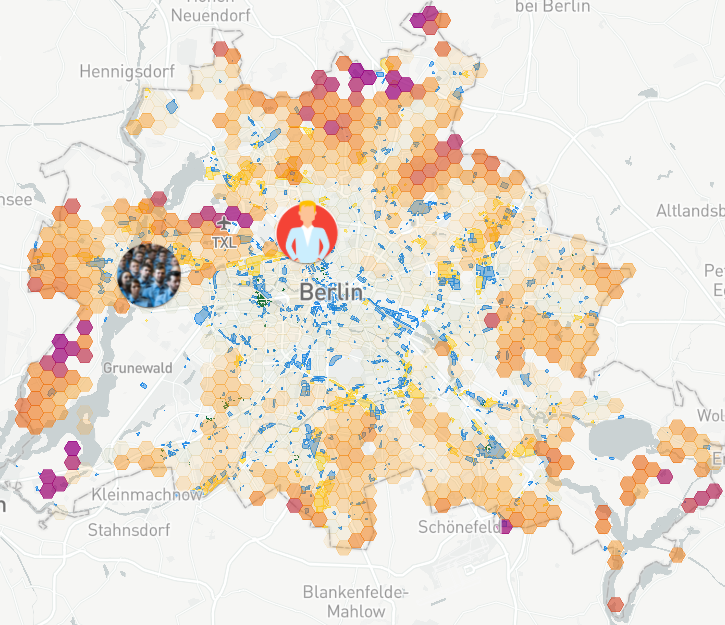
\includegraphics[width=7cm]{persona-spandau-01}
    \end{subfigure}%
    \begin{subfigure}{.5\textwidth}
        \centering
        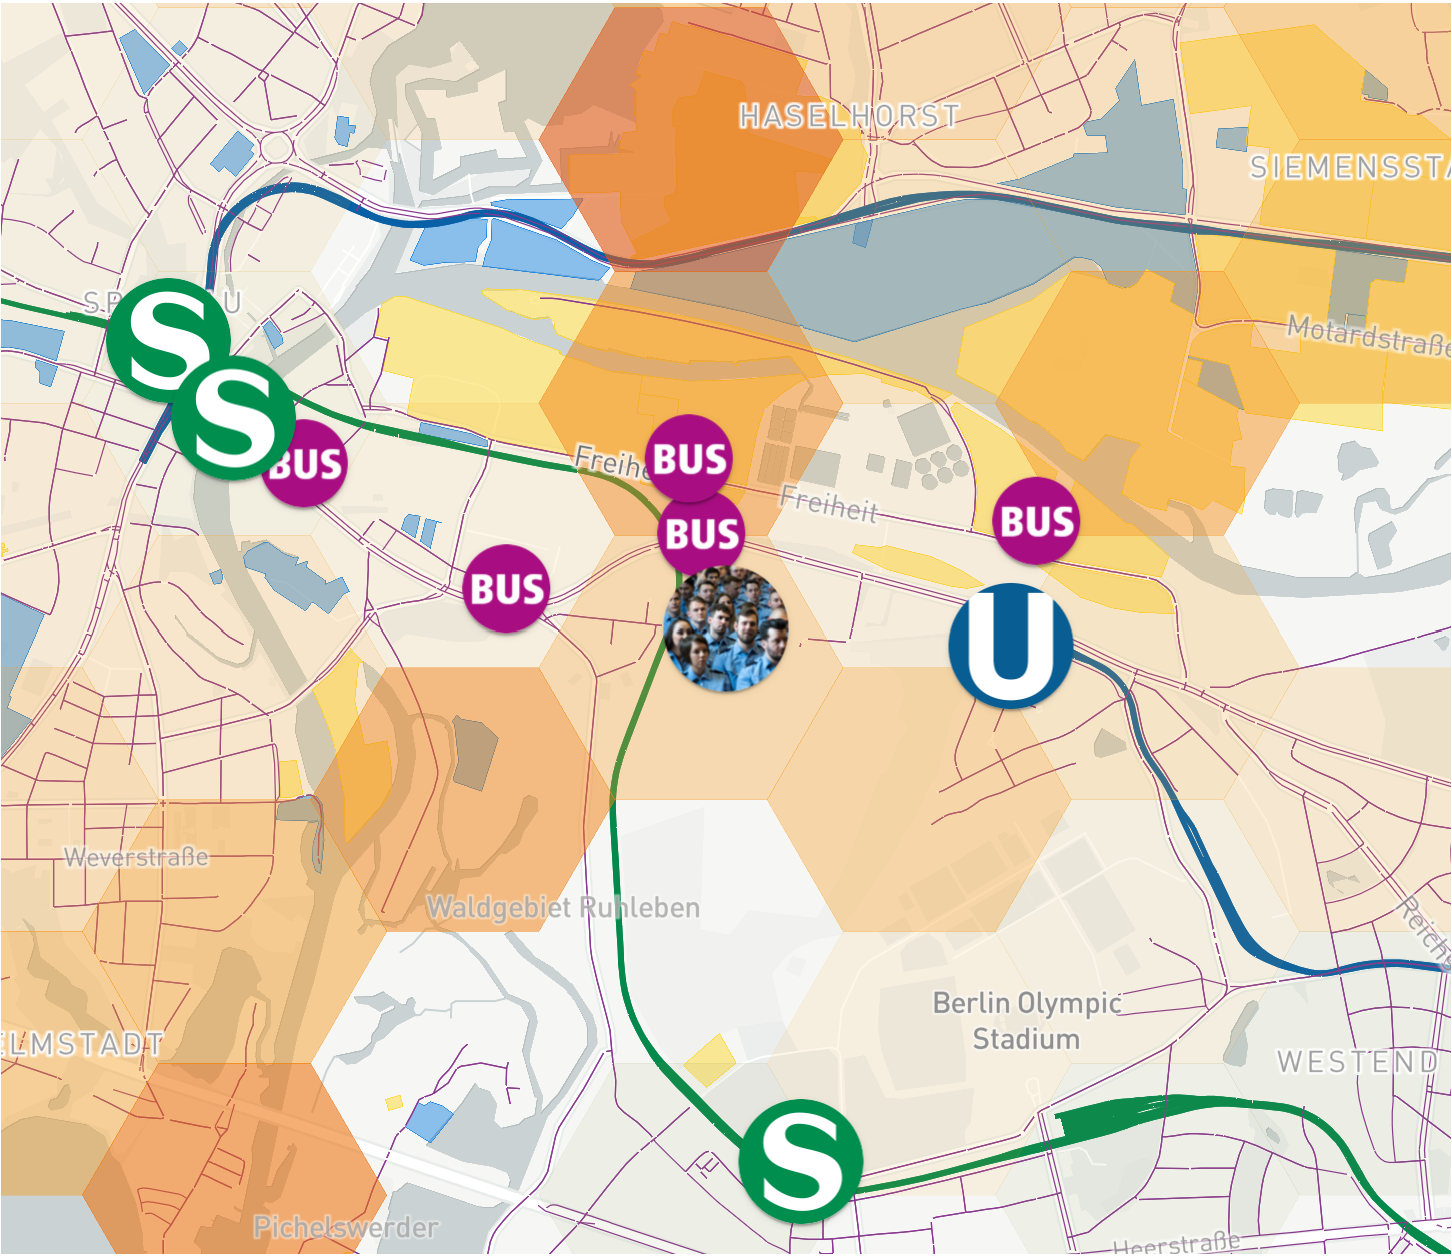
\includegraphics[width=7cm]{persona-spandau-02}
    \end{subfigure}
    \caption{Persona Industriestandort Spandau}
    \label{persona-spandau}
\end{figure}

Für den motorisierten Individualverkehr und den Busverkehr bildet der verlängerte Spandauer Damm die Hauptverkehrsader. Durch das hohe Pendleraufkommen reduziert sich jedoch die Durchschnittsgeschwindigkeit des Verkehrs gerade zu den Stoßzeiten merklich.

Trotz des hohen Verkehrsaufkommens stellen weder U-Bahn noch S-Bahn wegen ihrer großen Entfernung eine praktikable Alternative dar. Die nächste U-Bahnstation (Ruhleben) ist 22~Gehminuten entfernt und bildet mit der U2 eine direkte Verbindung unter anderem zum Zoologischen Garten und zum Alexanderplatz. Die nächste S-Bahnstation (Stresow) befindet sich 33 Gehminuten entfernt und bindet die S-Bahnlinien S9 und S3 sowie den Regionalbahnverkehr an. Fußläufig sind lediglich die Buslinien 131 und M45 erreichbar. Die unterschiedliche Taktung der Bus- und Bahnlinien verhindert jedoch ein schnelles Umsteigen, was sich negativ auf die Attraktivität des Busverkehrs auswirkt.

\paragraph{Lösungsansatz: Verbesserte S-Bahn Anbindung}
Um diesen Umstand zu ändern sieht der Berliner Nahverkehrsplan bereits eine Taktverdichtung des S-Bahnverkehrs auf den Linien S3 und S9 in Spandau vor.\footcite{NahverkehrsplanBerlin} Damit die Bahnverbindungen trotz des weiten Fußwegs als Option für mehr Pendler infrage kommen, sollten Busse eingesetzt werden, um eine direkte Verbindung zu den Bahnstationen herzustellen. Zu den Stoßzeiten sollten diese Busse regelmäßig verkehren, um die Wegzeit der letzten Meile so stark wie möglich zu verkürzen. Außerhalb der Stoßzeiten sollten die Busse als Rufbusse eingesetzt werden, um eine adäquate Anbindung auch während des Schichtbetriebs der angrenzenden Industrie zu gewährleisten.

\subsubsection{Urban Tech Republic - TXL}
\paragraph{Detailbetrachtung der Verkehrsinfrastruktur an der Urban Tech Republic - TXL}
Aufgrund der Mischung aus Wohn- und Gewerbegebiet entsteht in Charlottenburg-Nord viel Pendelverkehr. Nahe dem ehemaligen Flughafen TXL sind große Logistik- und Import-/Export-Unternehmen wie DPD, DB-Schenker und TNT ansässig. Die Einwohnerdichte von Charlottenburg-Nord liegt im Durchschnitt der Stadt.

Trotz geografischer Nähe zur Ringbahn weist dieses Gebiet durch eine geringe Stationsdichte eine schlechte Anbindung an den ÖPNV auf. Lediglich die Buslinie~128 ist fußläufig erreichbar. Um zur nächsten S-Bahnstation (Beusselstraße) zu gelangen, muss ein Fußweg von 28~Minuten zurückgelegt werden. Zur nächsten U-Bahnstation (Jakob-Kaiser-Platz) beträgt der Fußweg sogar 30~Minuten. Die direkte Anbindung an die Stadtautobahn ermöglicht außerhalb der Stoßzeiten eine sehr gute Verbindung mit dem motorisierten Individualverkehr. Auch während des verstärkten Verkehrsaufkommens in den Morgen- und Abendstunden bietet der Individualverkehr die schnellste Verbindung.

\begin{figure}
    \centering
    \begin{subfigure}{.5\textwidth}
        \centering
        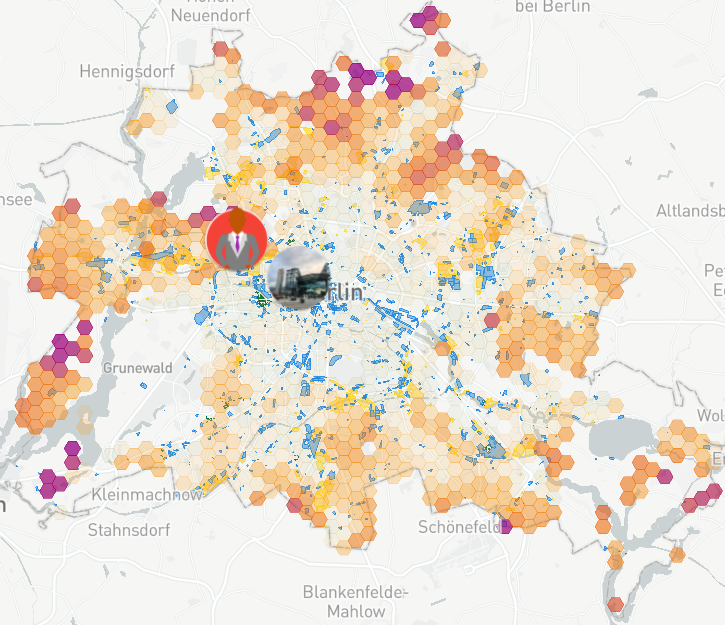
\includegraphics[width=7cm]{persona-charlottenburg-01}
    \end{subfigure}%
    \begin{subfigure}{.5\textwidth}
        \centering
        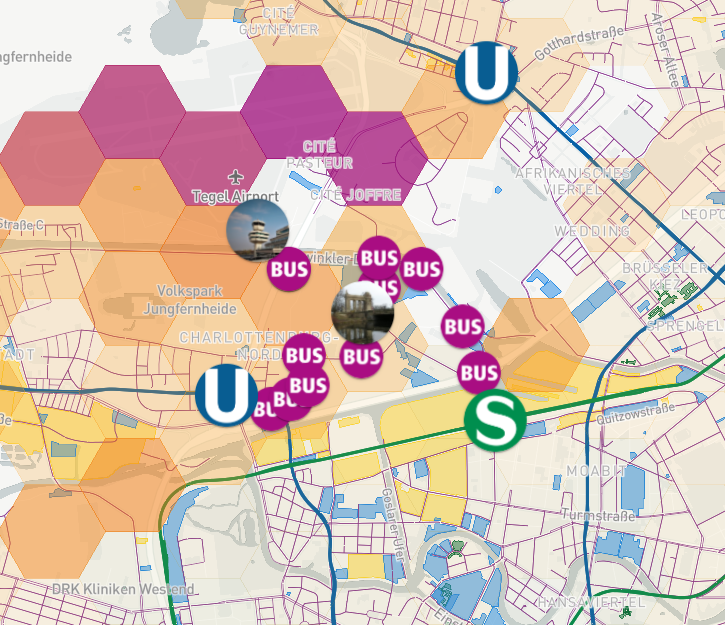
\includegraphics[width=7cm]{persona-charlottenburg-03}
    \end{subfigure}
    \caption{Persona Urban Tech Republic - TXL}
    \label{persona-charlottenburg-nord}
\end{figure}

Als besondere Herausforderung für den Verkehr in Charlottenburg-Nord gilt der Ausbau des ehemaligen Flughafens TXL zum Innovations- und Entwicklungsstandort. Durch die große Anzahl neuer Arbeitsplätze, die hier entstehen sollen, wird prognostiziert, dass das Verkehrsaufkommen merklich steigen wird.\footcite{UrbanTechRepublic} Aufgrund der Begrenzung durch den Berlin-Spandauer-Schifffahrtskanal im Norden und Osten sowie durch den Westhafenkanal im Süden gestaltet sich die Anbindung an die vorhandene Verkehrsinfrastruktur in angrenzenden Gebieten als schwierig.

\paragraph{Lösungsansatz 1: Anbindung mittels Ruf- und Pendelbus}
Aufgrund der geografischen Einschränkungen durch die Schifffahrtskanäle in Charlottenburg-Nord können bestehende Bus- oder Bahnlinien nicht so umgeplant werden, dass sinnvolle Verbindungen zu den vorhandenen Bahnstationen realisiert werden können. Stattdessen würde eine Kombination aus einem Pendelbusangebot während der Stoßzeiten und einem Rufbusangebot (zwischen den Stoßzeiten) bestehende Anschlusslücken schließen. Indem die Busse bestehende Bahnstationen direkt mit den abgeschnittenen Gebieten verbinden, entsteht eine schnelle Verbindung zur Ringbahn. Auf diese Weise könnte die Anbindungsqualität des ÖPNV in Charlottenburg-Nord signifikant gesteigert werden.

\paragraph{Lösungsansatz 2: Ausbau des Straßenbahnnetzes}
Um den zukünftigen Innovationsstandort Urban Tech Republic an das bestehende ÖPNV-Netz anzubinden, ist der Ausbau des Straßenbahnnetzes vom Kurt-Schumacher-Platz in Richtung Siemensstadt und Jakob-Kaiserplatz geplant.\footcite{NahverkehrsplanBerlin} Mittels einer Verbindung, die über das Gebiet des ehemaligen Flugfeldes laufen soll, wird der Entwicklungsstandort direkt angebunden. Durch die Einschränkungen der Schifffahrtskanäle steigern die entstehenden Haltestellen die Mobilität für die weiteren ansässigen Gewerbe jedoch kaum, da sie ebenfalls nur mit einem Fußweg von über 15~Minuten verbunden sind.

\subsubsection{Gewerbe- und Industriegebiet Landsberger Allee}
\paragraph{Detailbetrachtung der Verkehrsinfrastruktur am Gewerbe- und Industriegebiet Landsberger Allee}
Die Gegend rund um die Landsberger Allee, zwischen den Querstraßen Weißenseer Weg und Rhinstraße ist gekennzeichnet durch eine Vielzahl von Gewerbeflächen und Industrieanlagen. Zu den markantesten Einkaufsmöglichkeiten zählen das IKEA Einrichtungshaus, der Baumarkt Globus und das Dong Xuan Center. An der Landsberger Allee und den angrenzenden Querstraßen sind zudem zahlreiche Unternehmen aus den Bereichen Lebensmittelhandel, Maschinenbau und Automobilindustrie, sowie diverse Autovermietungen angesiedelt. Der öffentliche Nahverkehr ist in dieser Gegend auf senkrecht zueinander verlaufenden Straßenbahnlinien beschränkt.

\begin{figure}
    \centering
    \begin{subfigure}{.5\textwidth}
        \centering
        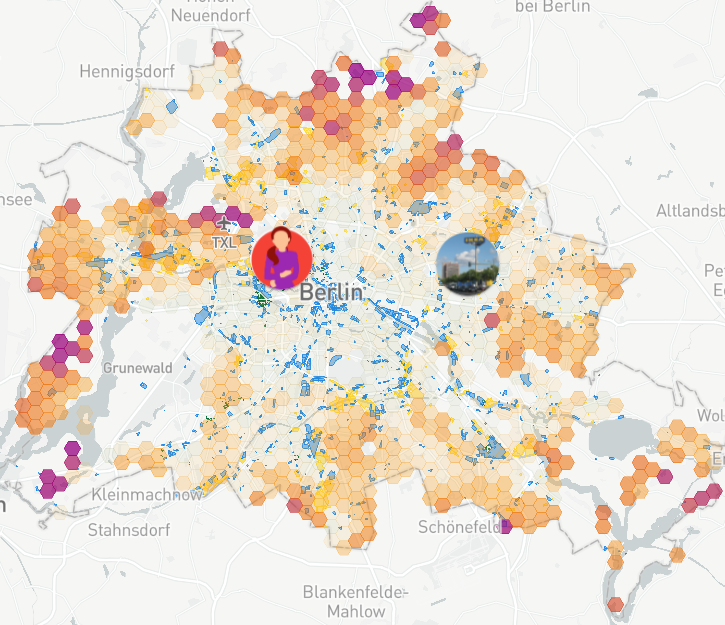
\includegraphics[width=7cm]{persona-landsberger-01}
    \end{subfigure}%
    \begin{subfigure}{.5\textwidth}
        \centering
        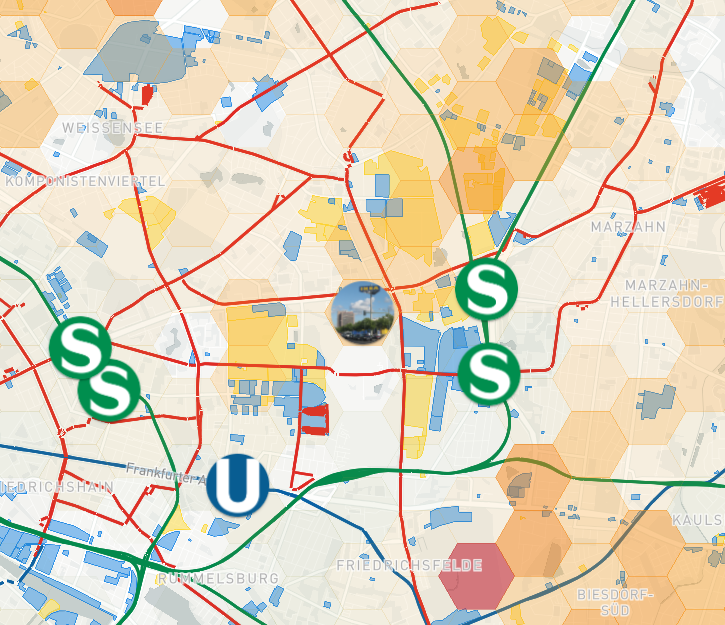
\includegraphics[width=7cm]{persona-landsberger-03}
    \end{subfigure}
    \caption{Persona Gewerbe- und Industriegebiet Landsberger Allee}
    \label{persona-landsberger-allee}
\end{figure}

Eine Anbindung an die Innenstadt bieten als weitere Verkehrsmittel des ÖPNV die U-Bahn-Station Magdalenenstraße, sowie die S-Bahn-Stationen Landsberger Allee, Storkower Straße, Springpfuhl und Pölchaustraße. Allerdings sind diese nicht fußläufig erreichbar. Insbesondere außerhalb der Stoßzeiten sind diese bedingt durch den geringeren Takt der Straßenbahn nur schwer zu erreichen.

\paragraph{Lösungsansätze}
Um die Anbindung an die anderen Verkehrsmittel des öffentlichen Nahverkehrs zu erhöhen, könnte zunächst eine Erhöhung der Taktung der Straßenbahn veranlasst werden. Zusätzlich könnte eine Nachtbuslinie eingerichtet werden, um die stark verringerte Taktung der Straßenbahn zwischen 0:00 und 07:00 Uhr zu kompensieren. Durch die Einrichtung eines Mobilitäts-Hubs (Jelbi Station) könnten beispielsweise Leihfahrräder zur Verfügung gestellt werden um die Wegzeit zur nächsten S- oder U-Bahn-Station zu verringern. Gegebenenfalls könnte ein solcher Mobilitäts-Hub auch durch die Kooperation mehrerer ortsansässiger Unternehmen realisiert werden.

\subsubsection{Der dicht besiedelte Osten Marzahn-Hellersdorfs}
\paragraph{Detailbetrachtung der Verkehrsinfrastruktur im dicht besiedelte Osten Marzahn-Hellersdorfs}
Der östliche Teil Marzahn-Hellersdorfs ist von einer sehr hohen Einwohnerdichte geprägt. Gleichzeitig existiert keine vielfältige Verkehrsinfrastruktur. Die ÖPNV-Anbindung in diesem Gebiet ist stark von der Straßenbahninfrastruktur geprägt. Die Straßenbahnhaltestellen Alte-Hellerdorfer und Michendorfer Straße bieten eine gute Anbindung innerhalb des Kiezes, Gebiete die außerhalb des Straßenbahnnetzes liegen, sind vom östlichen Rand Marzahn-Hellersdorfs jedoch kaum erreichbar. Die nächste S-Bahnstation Mehrower Allee ist mit dem Bus 30~Minuten entfernt. Der nächstgelegene U-Bahnhof Hellersdorf ist selbst mit dem Bus oder der Tram mindestens 15~Minuten entfernt.

\begin{figure}
    \centering
    \begin{subfigure}{.5\textwidth}
        \centering
        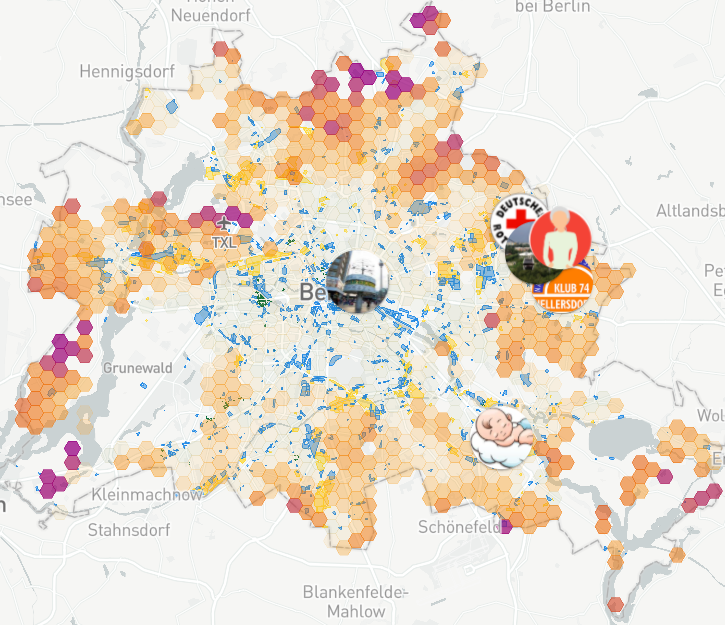
\includegraphics[width=7cm]{persona-marzahn-01}
    \end{subfigure}%
    \begin{subfigure}{.5\textwidth}
        \centering
        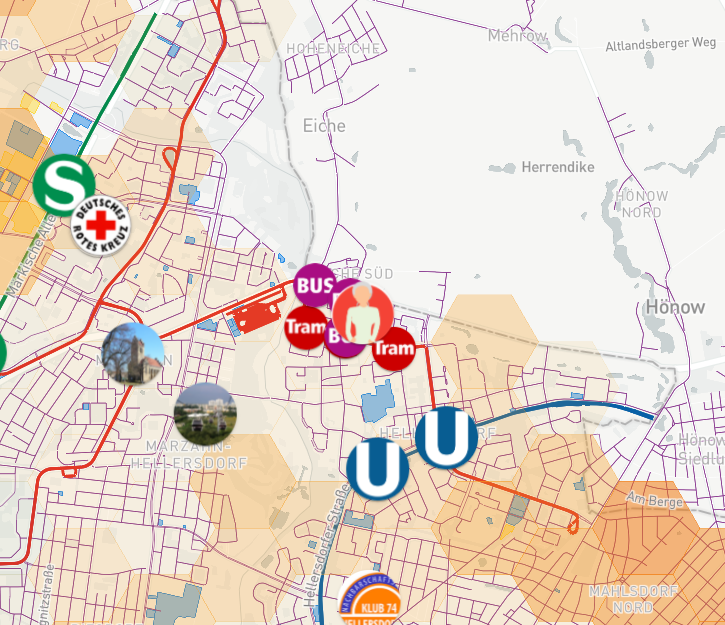
\includegraphics[width=7cm]{persona-marzahn-02}
    \end{subfigure}
    \caption{Der dicht besiedelte Osten Marzahn-Hellersdorfse}
    \label{persona-marzahn-hellersdorf}
\end{figure}

Von der aktuellen Verkehrssituation sind Arbeitnehmer*innen die in anderen Bezirken tätig sind besonders betroffen. Aber auch Senior*innen die sich innerhalb des Bezirks bewegen und beispielsweise in der Nachbarschaft engagieren, stehen vor großen Herausforderungen. Wichtige Begegnungsstätten, wie das Deutsche Rote Kreuz und der Nachbarschaftshilfe Klub~74~e.V. sind mit dem ÖPNV nicht in unter 30~Minuten erreichbar. Weitere Wege, beispielsweise bis zum Alexanderplatz, sind zwar mit der Straßenbahn erreichbar, setzen aber eine Reisezeit von mindestens 45 Minuten voraus.

\paragraph{Lösungsansätze}
Um die Erreichbarkeit innerhalb des Bezirks zu verbessern, sollte die Taktung der bestehenden Bus- und Straßenbahn Linien erhöht werden. Um die Anbindung an das übrige Stadtgebiet zu stärken, sollte die Anbindung an die S-Bahnstation Mehrower Allee und den U-Bahnhof Hellersdorf verbessert werden. Zu diesem Zweck könnten Expressbus-Linien eingerichtet werden, die die bestehende ÖPNV-Infrastruktur besser verknüpft.

\subsubsection{Gewerbegebiet Gradestraße}
\paragraph{Detailbetrachtung der Verkehrsinfrastruktur am Gewerbegebiet Gradestraße}
Anhand der genaueren Betrachtung von Gewerbedichte und Lücken innerhalb der Verkehrsinfrastruktur konnte das Gewerbegebiet an der Gradestraße, Ecke Tempelhofer Weg identifiziert werden. In diesem Gewerbegebiet im nördlichen Britz, sind international agierende Unternehmen und wichtige Arbeitgeber wie Kieback\&Peter GmbH, Linde Gas Deutschland und Terra Naturkost Handels KG angesiedelt. Zusätzlich zur hohen Industrie- und Gewerbedichte, weist das Gebiet eine verhältnismäßig hohe Einwohnerdichte auf. Die Verkehrsanbindung des Gewerbegebiets Gradestraße ist jedoch mangelhaft.

\begin{figure}
    \centering
    \begin{subfigure}{.5\textwidth}
        \centering
        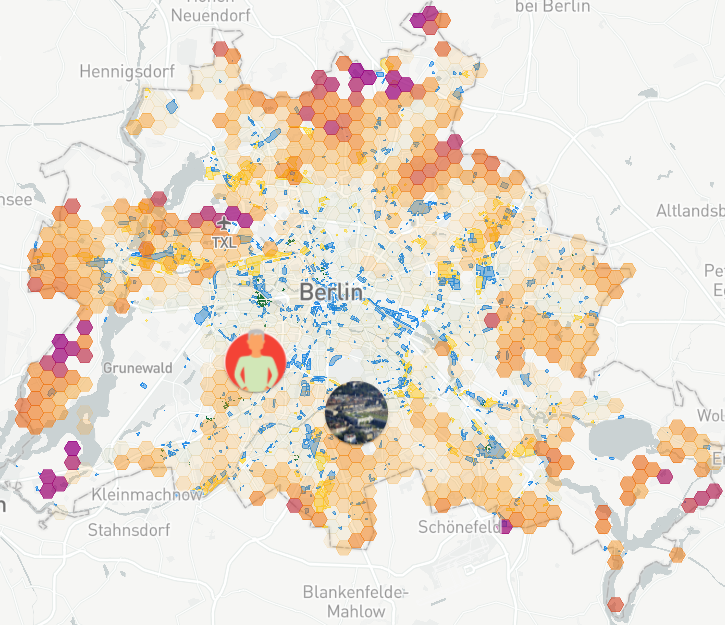
\includegraphics[width=7cm]{persona-britz-01}
    \end{subfigure}%
    \begin{subfigure}{.5\textwidth}
        \centering
        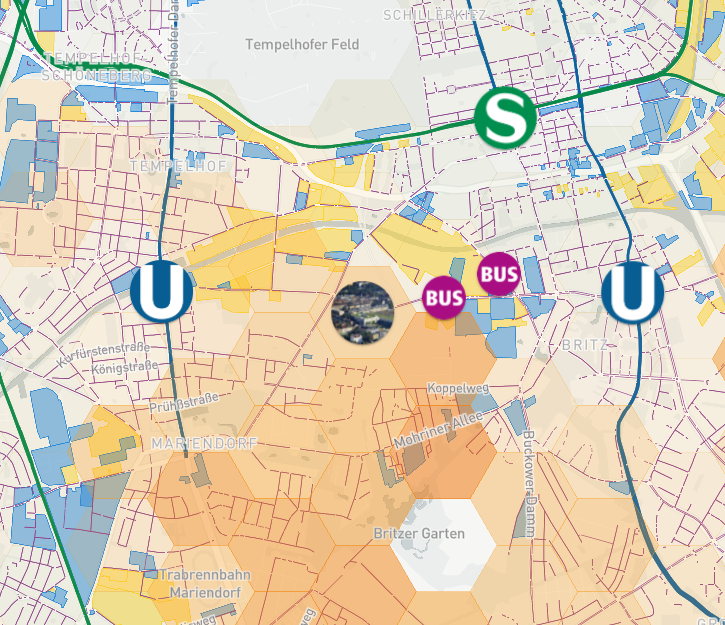
\includegraphics[width=7cm]{persona-britz-02}
    \end{subfigure}
    \caption{Gewerbegebiet Gradestraße}
    \label{persona-britz}
\end{figure}

Die Erreichbarkeit des Gewerbegebiets Gradestraße ist stark von der guten Anbindung an die Stadtautobahn abhängig. Der ÖPNV ist in der Nähe des Gewerbegebiets nur unzureichend ausgebaut. Ausgehend von dem Gewerbegebiet sind die Buslinien 170 und M44 fußläufig erreichbar. Die Buslinie 170 wird außerhalb der Stoßzeiten nur im 20~Minuten-Takt bedient und selbst die regelmäßiger verkehrende Linie M44 bietet keine ausreichende Anbindung an den ÖPNV. Die U-Bahnstationen Blaschkoallee und Ullsteinstraße sind je 26 ~ehminuten und 9~Bus-Minuten entfernt. Die nächste S-Bahnstation (Hermannstraße) ist sogar 32~Gehminuten entfernt. Selbst mit dem Bus M44 ist die S-Bahnstation Hermannstraße, aufgrund von vier Zwischenhalten 17~Minuten entfernt.

\paragraph{Lösungsansatz 1: Erhöhte Taktung und neue Buslinie}
Aktuell gibt es in Britz und dem Raum Gradestraße keine laufenden oder geplanten Infrastrukturprojekte.\footcite{NahverkehrsplanBerlin} Damit die Anbindung des Gewerbegebiets verbessert werden kann, sollte zunächst die Erreichbarkeit der bestehenden ÖPNV-Infrastruktur verbessert werden. Durch eine erhöhte Taktung des Busverkehrs außerhalb der Stoßzeiten wäre es möglich, dass im Schichtsystem tätige Arbeitnehmer*innen den ÖPNV anstelle des Individualverkehrs nutzen können. Zusätzlich könnte die Einführung einer neuen Express-Linie in Richtung der S-Bahnstation Hermannstraße die Wegzeit deutlich verkürzen. Auf diese Weise könnte die Attraktivität des ÖPNV deutlich gesteigert werden.

\paragraph{Lösungsansatz 2: Ausbau des Straßenbahnnetzes}
Im Nahverkehrsplan des Landes Berlin wird zumindest der Bedarf zum Ausbau des Straßenbahn-Netzes im Süden des Bezirks Neukölln identifiziert. Die konkrete Planung des Vorhabens steht noch aus, könnte aber tatsächlich zu einer deutlichen Verbesserung der Verkehrssituation in der Nähe des Gewerbegebiets Gradestraße beitragen.\footcite{NahverkehrsplanBerlin}

\newpage

\section{Ergebnispräsentation (Arbeitspaket 4)}
\label{ergebnispraesentation}

Die Analyseergebnisse werden in Form von interaktiven Karten und begleitenden Texten miitels einer Webapplikation zur Verfügung gestellt. Die Webapplikation ist unter der URL \url{https://berlin-mobility.web.app} für die Öffentlichkeit zugänglich. Die Grundlage der Webapplikation bildet das quelloffene Webapplikationsframework Angular\footnote{https://angular.io/}, welches in Version 10 zum Einsatz kommt.

\img{app-01-landing-page}{app-01-landing-page}{width=14cm}{Startseite der Webapplikation}

Die Webapplikation ist in zwei Bereiche unterteilt, welche im Folgenden beschrieben werden.

\begin{itemize}
    \item Die \emph{Story} stellt die Ergebnisse der Arbeitspakete 1-3 dar.
    \item Das \emph{Dashboard} ermöglicht der Leser*in die Daten selbst zu erkunden indem, in einer Karte interaktiv Ebenen ein- und ausgeblendet werden können.
\end{itemize}

\subsection{Visualisierung der Analyseergebnisse}
\label{visualisierung_der_analyseergebnisse}

Innerhalb der \emph{Story} stellt geht die Navigation ausschließlich von der Betätigung des Mausrads aus. Durch scrollen kann sich die Leser*in durch die Abschnitte bewegen. Gleichzeitig werden durch das Scrollen Informationsebenen (sogenannte Overlays) auf den Karten geändert und Animationen ausgelöst. Um der Leser*in eine Einführung in das Thema zu geben, werden zunächst die Hintergründe des Projekts beschrieben. Dabei werden sowohl das Berlin Mobilitätsgesetz, als auch die daran geäußerte Kritik ausgeführt.

Im zweiten Abschnitt werden die Analyseergebnisse des Arbeitspakets 1 aufbereitet (siehe Kapitel~\ref{arbeitspaket_1_beschreibung_der_ist_situation}). Dabei wird eine Kombination aus Kartenmaterial, Overlays, Marker und erklärendem Text genutzt. Durch scrollen kann sich die Leser*in im Text bewegen. Das Kartenmaterial sowie die Overlays und Marker passen sich dabei immer den sichtbaren textlichen Inhalten an. Die Interaktionsmöglichkeiten für die Leser*in sind bewusst gering gehalten. Neben der Möglichkkeit zu scrollen, können Leser*innen Marker, durch Bewegen der Maus über relevante Textstellen, auf dem Kartenmaterial ein- und ausblenden.

Im dritten Abschnitt wird anhand zweier Beispiele die Bedeutung und Funktionsweise von Isochronen erläutert. Eine animierte Karte mit entsprechender Legende vermittelt der Leser*in anschaulich, wie sich Isochronen bei Veränderung des zeitlichen Parameters verändern. Ebenfalls wird ersichtlich, dass sich Isochronen verschiedener Verkehrsmittel deutlich voneinander unterscheiden.

Der vierte Abschnitt der \emph{Story} stellt die Ergebnisse des Arbeitspakets 2 dar (siehe Kapitel~\ref{arbeitspaket_2_aufzeigen_von_schwachstellen_der_vorhandenen_infrastruktur}), und befasst sich dementsprechend  mit den Schwachstellen des Berliner Verkehrsnetzes.

Zu Beginn des Abschnitts wird die in Kapitel~\ref{verkehrsmittelspezifische_analyse} beschreibene Vorgehensweise zur Berechnung der Anbindungsqualität vorgestellt. Die Analyseergebnisse werden mittels \emph{Turf}\footnote{http://turfjs.org/docs/\#hexGrid} zu Hexagonen aggregiert und farblich kodiert. Gut angebundene Gebiete sind  grün hinterlegt, schlecht angebundene Gebiete sind magentafarben gekennzeichnet. Anhand dieser einfachen Farbkodierung sind die Analysergebnisse auch für Laien leicht zugänglich.

Der Fokus des finalen Abschnitts liegt auf der Präsentation der Lösungsansätze (siehe Kapitel~\ref{arbeitspaket_3_ableiten_von_handlungsempfehlungen}). Zunächst wird das Priorisierungsverfahren erörtet, welches zur Auswahl der fünf adressierten Orte genutz wird. Die Lösungsansätze werden anhand von fünf Personas beschrieben. Dabei werden die zur jeweiligen Persona gehörigen Orte, Verkehrslinien und Haltestellen auf der Karte hervorgehoben. Ein dynamischer Zoom zentriert den Kartenausschnitt, der ausgehend von der jeweiligen Persona beschrieben ist.

\subsection{Interaktives Mobilitäts-Dashboard}
\label{interaktives_mobilitaets_dashboard}

Um der Kritik gefühlter Intransparenz, die in Kapitel~\ref{problems} beschrieben ist, entgegenzuwirken, wurde ein interaktives Dashboard entwickelt. Dieses Dashboard ermöglicht es Bürger*innen sich auch ohne spezifisches Vorwissen mit den Daten und Erkenntnissen zu beschäftigen, die als Grundlage der Mobilitätsentscheidungen des Senats dienen.

Auf mehreren Verkehrsmittelspezifischen Unterseiten und einer Seite mit verkehrsmittelübergreifenden Information haben Bürger*innen, Entscheider*innen sowie Städte*planerinnen die Möglichkeit über die Inhalte der \emph{Story} hinaus, Daten auf eigene Faust zu erkunden. Durch interaktive Elemente können Nutzer*innen beispielsweise die Verkehrssituation verschiedener Orte innerhalb der Stadt miteinander vergleichen.

Auf den folgenden Unterseiten haben Nutzer*innen die Möglichkeit direkt mit Mobiltiätsdaten zu interagieren:

\paragraph{Öffentlicher Personennahverkehr}

Auf dieser Seite werden alle Berliner Bus- und Bahnverbindungen des öffentlichen Nahverkehrs innerhalb von Berlin visualisiert. Darüber hinaus können Nutzer*innen auf einzelnen Ebenen die Erreichbarkeit der Stadt mittels aller öffentlichen Verkehrsmittel ein- und ausblenden.

\img{dashboard-opnv}{dashboard-opnv}{width=14cm}{Interaktives Dashboard öffentlicher Personennahverkehr}
\paragraph{Motorisierter Individualverkehr}

Auf dieser Seite können Nutzer*innen die Engstellen des Straßenverkehrs betrachten. Auf vier Kacheln werden die durchschnittlich tatsächlich gefahrenen Geschwindigkeiten, die Verteilung der maximal zulässigen Höchstgeschwindigkeiten innerhalb der Stadt, Stoßzeiten auf einer Zeitachse sowie die Erreichbarkeit mittels der 15-Minuten-Isochrone visualisiert.

\img{dashboard-miv}{dashboard-miv}{width=14cm}{Interaktives Dashboard motorisierter Individualverkehr}
\paragraph{Zukünftige Erweiterungen}

Um den Nutzer*innen der Webapplikation zukünftig einen noch breiteren sowie einfacheren Zugang zu Mobilitätsdaten zu ermögichen, werden weitere Dashboards entwickelt. In der Planung befindet sich beispielsweise ein Dashboard, dass sich mit dem geplante Tram-Netz beschäftigt, und ein Dashboard, dass auf den in Kapitel~\ref{mobwob_index} beschriebenen Mobilitätsindex eingeht.

\newpage

\section{Ergebnisreflexion}
\label{ergebnisreflexion}

Die in den vorangegangen Kapiteln beschriebenen Analyseansätze und Visualisierungsformen ergeben einen Prototypen für die datengetriebene Analyse und Gestaltung der Berliner Verkehrsinfrastruktur. Durch die gezielte Weiterentwicklung der Analyse sowie der zur interaktiven Datenexploration entwickelten Webapplikation, könnte ein umfangreiches Werkzeug für Städteplaner und die Berliner Senatsverwaltung für Umwelt, Verkehr und Klimaschutz geschaffen werden. Im Folgenden werden die Projektergebnisse zusammenfassend dargestellt. Ausgehend davon werden die Limitierungen des gewählten Ansatzes beschrieben und mögliche nächste Schritte skizziert.

\subsection{Zusammenfassung der Projektergebnisse}
Die in Kapitel~\ref{projekt_und_analyseergebnisse} gezeigten Analyseansätze ermöglichen eine detaillierte Analyse der in Bezug auf die stark variierende Anbindungsqualität im Stadtgebiet. Ausgehend von der Berechnung der durchschnittlichen Erreichbarkeit fest definierte Bereiche mithilfe von Isochronen, können Unterschiede in der Anbindungsqualität bzw. hinsichtlich der Qualität der vorhandenen Verkehrsinfrastruktur an unterschiedlichen Orten im Stadtgebiet offengelegt werden.

Aus den Ergebnissen geht deutlich hervor, dass die innerstädtischen Wohngebiete bereits gut angebunden sind. Bei der Anbindung von Industrie, Gewerbe und Handel gibt es dahingegen Handlungsbedarf. Zudem scheint in den Außenbezirken eine stärkere Verzahnung des bereits bestehenden ÖPNV Angebotes notwendig zu sein. Die Außenbezirke sind häufig auf einzelne Linien sowie einzelne Verkehrsmittel angewiesen.

\subsection{Limitierungen}\label{limitierung}
\subsubsection{Datenverfügbarkeit und Qualität}
Für die Analyse der Verkehrsinfrastruktur werden, wie in Kapitel \ref{projektumsetzung} beschrieben, hauptsächlich öffentlich zugängliche Geo- und Populationsdaten verwendet. Die genutzten Daten decken jedoch nicht den vollständigen Informationsbedarf für alle detaillierte Analysen, die im Zusammenhang mit innerstädtischer Mobilität durchgeführt werden können. Da diese fehlenden Daten jedoch nicht in ausreichender Qualität und zu mit dem Projektbudget zu vereinbaren Kosten verfügbar waren, leitet sich daraus eine Einschränkung des Analyseumfangs ab. Im Rahmen des Projekts wurden folgende Limitierungen des Analyseumfangs aufgrund mangelnder Datenverfügbarkeit identifiziert:

\begin{itemize}

    \item Die Anzahl der Beschäftigten die in den identifizierten Gewerbe-, Handels- und Industriegebieten tätig sind wird im Zuge der Analyse nicht berücksichtigt. Entsprechende Informationen werden nicht automatisiert erfasst, bzw. stehen nicht öffentlich zur Verfügung. Durch die Berücksichtigung von Beschäftigtenzahlen könnten Aussagen über das zu erwartende Auslastung der Verkehrsinfrastruktur in bestimmten Teilen des Stadtgebiets getroffen werden.

    \item Die Betrachtung der Auslastung des ÖPNV ist nicht Teil des aktuellen Projekts. Entsprechende Daten sind nicht öffentlich zugänglich. Die Betrachtung der aktuellen Auslastung ist für die Dimensionierung neuer ÖPNV-Vorhaben unerlässlich.

    \item Die Taktung des ÖPNV wird in der Analyse nicht berücksichtigt​. Eine zuverlässige und effiziente Einbindung entsprechender Daten waren aufgrund der limitierten Ressourcen im Rahmen des Projekts nicht möglich.

    \item Die Daten zu den tatsächlichen Geschwindigkeiten des Autoverkehrs liegen nicht für alle Straßenabschnitte/-segmente vor​. Durch die weitere Anreicherung der im Projekt genutzten Daten um weitere Straßensegmente, könnte eine die Analyse des Straßenverkehrs weiter detailliert werden.

    \item Die Barrierefreiheit von Haltestellen wird aufgrund fehlender Daten nicht berücksichtigt​. Die Verfügbarkeit entsprechender Daten ist die Voraussetzung dafür, dass bei der Berechnung der Anbindungsqualität auch die Bedürfnisse von Bürger*innen mit eingeschränkter Mobilität berücksichtigt werden können.

    \item Es werden weder Hausbote, noch gewerbliche Flächen und Verkehrsmittel auf Wasserflächen in der Analyse berücksichtigt. Insbesondere die durch die BVG betriebenen Fähren könnten im weiteren Verlauf in die Analyse mit aufgenommen werden, um den Detailgrad weiter zu steigern.

\end{itemize}

\subsubsection{Komplexität der Analyse}
Ausgehend von der limitierten Datenverfügbarkeit und -qualität sowie den limitierten Ressourcen ergeben sich auch hinsichtlich der Komplexität der Analyse Limitierungen.

\begin{itemize}
    \item Die Bestimmung der Anbindungsqualität wird im Rahmen des Projekts ausschließlich durch die Berechnung der Erreichbarkeit auf Basis von Isochronen vorgenommen. Durch die Anreicherung um die Taktung des ÖPNV sowie die Auslastung der vorhandenen Verkehrsinfrastruktur, würde die Anbindungsqualität weiter an Aussagekraft gewinnen.
    \item Bei der Berechnung der Anbindungsqualität werden keine „Penalty“ eingerechnet. So werden weder für die Nutzung des Autos Zeiten für die Parkplatzsuche, noch bei der Nutzung des ÖPNV Zeiten für Umstiege (bspw. für die Wegstrecke von einer U-Bahnlinie zu einer S-Bahnlinie) berücksichtigt.
    \item Aktuell werden basierend auf Heuristiken und Vorüberlegungen (siehe Kapitel \ref{vorbereitung}) ausschließlich 15-Minuten-Isochronen analysiert​. Die Berechnung von Isochronen ist ressourcenintensiv, sodass zwischen der Berechnung unterschiedlicher Isochronen abgewogen werden musste.
\end{itemize}

\subsubsection{Begrenztes Domänenwissen}
Im Rahmen des Projekts wurden Expert*innen der Senatsverwaltung für Umwelt, Verkehr und Klimaschutz punktuell in die Entwicklung des Prototyps eingebunden. Für die Weiterenwicklung des Analyseansatzes ist eine stärkere Einbeziehung von Domänenwissen notwendig. Entsprechendes Domänenwissen wird auch auch für die Validierung der in Kapitel~\ref{projekt_und_analyseergebnisse} vorgestellten Handlungsvorschläge vorausgesetzt.

\subsection{Ausblick}

\subsubsection{Anreicherung der Analyse}
Die Anreicherung der Analyse - ausgehend von den in den Kapiteln 5.2.1 und 5.2.2 beschriebenen Limitierungen - würde die  Genauigkeit der Prädiktionen der Analyse weiter steigern. Demnach sollte eine Erweiterung der Datengrundlage sowie eine Steigerung der Analysekomplexität angestrebt werden. Insbesondere die Berücksichtigung von Datenpunkten bezüglicher der Taktung und Auslastung des ÖPNV wäre zielführend. Zudem würde die Einbindung von „Penalties“ (bspw. Zeit für die Parkplatzsuche bei Nutzung eines PKW) eine Feinjustierung des Analyseansatzes ermöglichen.

\subsubsection{Finalisierung des interaktiven Mobililitätskompasses}
Wie in Kapitel \ref{ergebnispraesentation} beschrieben, verfügt der Prototyp bereits heute über einen interaktiven Modus. Mithilfe des interaktiven Mobilitätskompasses, bzw. Dashboards lassen sich individuelle Analysen der Verkehrsinfrastruktur durchführen. In Kapitel \ref{problems} wird dargelegt, dass die fehlende Einbindung der Bürger*innen zu Kritik an der Umsetzung des Mobilitätsgesetzes führt. Durch den gezielten Ausbau des interaktiven Mobilitätskompasses könnte ein Werkzeug für die die Bürger*innenkommunikation geschaffen werden, welches von Bürger*innen genutzt werden könnte um sich über den aktuellen Stand der Verkehrsinfrastrukutr zu erkundigen. Auf diese Weise könnten Bürger*innen die Notwendigkeit einzelner Infrastrukturmaßnahmen gezielt nachvollziehen. Es könnte auch ein Votingsystem zur Priorisierung von Infrastrukturmaßnahmen eingeführt werden, um das Gefühl der Teilhabe zu steigern.


\img{app-dashboard}{app-dashboard}{width=14cm}{Individuelles Dashboard (eigene Darstellung)}

\subsubsection{Entwicklung eines Planungstools}
Der interaktive Mobilitätskompass dient zudem als Ausgangspunkt für die Entwicklung eines umfangreichen Planungstools für Städteplaner und Entscheider*innen in der Berliner Senatsverwaltung für Umwelt, Verkehr und Klimaschutz. Zusätzlich zu der deskriptiven Analyse der Ist-Situation könnten beispielsweise Streckenverläufe, die sich noch in der Planung befinden, in die Graphen-Struktur eingepflegt werden. Auf diese Weise könnte simuliert werden, wie sich die Realisierung eines bestimmten Infrastrukturprojekts (bspw. die Erweiterung einer S-Bahnstrecke) auf die Anbindungsqualität im betroffenen Stadtgebiet auswirken würde. Dadurch könnten die Potenziale von Infrastrukturvorhaben unkompliziert und visuell evaluiert werden.

\subsubsection{Entwicklung eines Mobilitätsindexes}\label{mobwob_index}
Durch die fortlaufende Erweiterung und Aktualisierung der Datengrundlage könnte auf Basis des in den Kapiteln~\ref{projektumsetzung} und \ref{projekt_und_analyseergebnisse} vorgestellten Analyseansatzes ein fortlaufender Mobilitätsindex entwickelt werden. Unter Berücksichtigung relevanter Faktoren wie Handels-, Industrie- und Gewerbedichte, Einwohnerdichte, Taktung, Verfügbarkeit und Geschwindigkeit könnten der Mobilitätsindex eingesetzt werden um Veränderungen in der Anbindungsqualität über die Zeit feststellen zu können und um weitere Maßnahmen zu identifizieren. 

Die Entwicklung eines Mobilitätsindexes mit Fokus auf die durch die Verkehrsinfrastruktur gewährleistete Anbindungsqualität, wäre eine wertvolle Ergänzung zum bestehenden Bundesländerindex Mobilität \& Umwelt.\footcite{Bundeslaenderindex:1}

Der Bundesländerindex Mobilität \& Umwelt bewertet die Verkehrsinfrastruktur auf Ebene der Bundesländer entlang der Faktoren Verkehrssicherheit, Lärmminderung, Flächenverbrauch, Klimaschutz und Luftqualität (siehe Abbildung~\ref{mob-index2020}).

\img{mob-index2020}{mob-index2020}{width=14cm}{Bundesländerindex Mobilität \& Umwelt Ergebnisse \footcite{Bundeslaenderindex:1}}

Analog zum Bundesländerindex Mobilität \& Umwelt könnte der Mobilitätsindex durch eine entsprechende Anreicherung der Datengrundlage dahingehend ausgestaltet werden, dass der laufende Vergleich (Monitoring) der Anbindungsqualität auf Ebene der Bundesländer oder Städte möglich ist.

\img{mob-index2018-Verteilung}{mob-index2018-Verteilung}{width=14cm}{Bundesländerindex Mobilität \& Umwelt Gewichtung \footcite{Bundeslaenderindex:1}}

Die gezeigte Verteilung verdeutlicht wie der Bundesmobilitätsindex gewichtet wurde. Es wird dazu konstruktiv der folgende Vorschlag unterbreitet, der nur ein Minimum an Ergänzungen darstellt.

\img{mob-index-anpassung}{mob-index-anpassung}{width=14cm}{Mobilitätsindex ergänzt und erweitert (eigene Darstellung)}

Die in Abbildung~\ref{mob-index-anpassung} dargestellte Erweiterung sieht unter anderem eine andere Gewichtung vor. Vor allem sollten die genutzten Flächen einen höheren Beitrag zur Bewertung aufweisen. Dies könnte die Korrelation zwischen dicht besiedelten Gebieten und der Luftqualität abschwächen aber auch die CO2 Emittierung von dichten Industrieansiedlungen in dem Bundesland oder dem Stadtstaat.
Am wichtigsten ist aber mitunter das Einführen einer neuen Datenquelle bzw. einer neuen Dimension. Der öffentliche Nahverkehr und der regionale Überlandverkehr ist besonders in nicht dicht besiedelten Gebieten essentiell.
Das Abbilden des Ausbaus der Nutzung etc. zeigt in einem stetigen Mobilitätsindexes auch deren Entwicklung an und kann als Werkzeug zur Transparenz genutzt werden.
Des Weiteren lassen sich mit einer immer komplexeren Formalisierung eines ganzheitlichen Indexes Städte, Bundesländer oder sogar Landkreise vergleichen. Dies ermöglicht Planer*innen aber auch Förderer*innen, Mittel und Maßnahmen an den geeigneten Stellen zu platzieren.

%\section{Fazit}
Wünsche Euch allen viel Erfolg für das 7. Semester und bei der Erstellung der Thesis. Über Anregungen und Verbesserung an dieser Vorlage würde ich mich sehr freuen. 


%-----------------------------------
% Apendix / Anhang
%-----------------------------------
%\newpage
%\section*{\AppendixName} %Überschrift "Anhang", ohne Nummerierung
%\addcontentsline{toc}{section}{\AppendixName} %Den Anhang ohne Nummer zum Inhaltsverzeichnis hinzufügen
%
%\begin{appendices}
%% Nachfolgende Änderungen erfolgten aufgrund von Issue 163
%\makeatletter
%\renewcommand\@seccntformat[1]{\csname the#1\endcsname:\quad}
%\makeatother
%\addtocontents{toc}{\protect\setcounter{tocdepth}{0}} %
%	\renewcommand{\thesection}{\AppendixName\ \arabic{section}}
%	\renewcommand\thesubsection{\AppendixName\ \arabic{section}.\arabic{subsection}}
%	\section{Beispielanhang}\label{Beispielanhang}
Dieser Abschnitt dient nur dazu zu demonstrieren, wie ein Anhang aufgebaut seien kann.
\subsection{Weitere Gliederungsebene}
Auch eine zweite Gliederungsebene ist möglich.
\section{Bilder}
Auch mit Bildern.
Diese tauchen nicht im Abbildungsverzeichnis auf.
\begin{figure}[H]
    \centering
    \caption[]{Beispielbild}
	\label{fig:Beispielbild}
    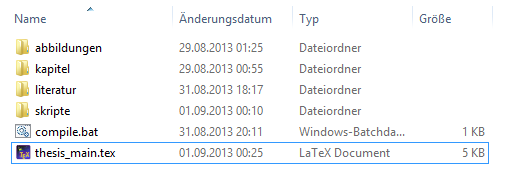
\includegraphics[width=1\textwidth]{verzeichnisStruktur}
\end{figure}
%\end{appendices}
%\addtocontents{toc}{\protect\setcounter{tocdepth}{2}}

%-----------------------------------
% Literaturverzeichnis
%-----------------------------------
\newpage

% Die folgende Zeile trägt ALLE Werke aus literatur.bib in das
% Literaturverzeichnis ein, egal ob sie zietiert wurden oder nicht.
% Der Befehl ist also nur zum Test der Skripte sinnvoll und muss bei echten
% Arbeiten entfernt werden.
%\nocite{*}

%\addcontentsline{toc}{section}{Literatur}

% Die folgenden beiden Befehle würden ab dem Literaturverzeichnis wieder eine
% römische Seitennummerierung nutzen.
% Das ist nach dem Leitfaden nicht zu tun. Dort steht nur dass 'sämtliche
% Verzeichnisse VOR dem Textteil' römisch zu nummerieren sind. (vgl. S. 3)
%\pagenumbering{Roman} %Zähler wieder römisch ausgeben
%\setcounter{page}{4}  %Zähler manuell hochsetzen

% Ausgabe des Literaturverzeichnisses

% Keine Trennung der Werke im Literaturverzeichnis nach ihrer Art
% (Online/nicht-Online)
%\begin{RaggedRight}
%\printbibliography
%\end{RaggedRight}

% Alternative Darstellung, die laut Leitfaden genutzt werden sollte.
% Dazu die Zeilen auskommentieren und folgenden code verwenden:

% Literaturverzeichnis getrennt nach Nicht-Online-Werken und Online-Werken
% (Internetquellen).
% Die Option nottype=online nimmt alles, was kein Online-Werk ist.
% Die Option heading=bibintoc sorgt dafür, dass das Literaturverzeichnis im
% Inhaltsverzeichnis steht.
% Es ist übrigens auch möglich mehrere type- bzw. nottype-Optionen anzugeben, um
% noch weitere Arten von Zusammenfassungen eines Literaturverzeichnisse zu
% erzeugen.
% Beispiel: [type=book,type=article]
\printbibliography[type=online,heading=bibintoc,title={\langde{Literaturverzeichnis}\langen{Bibliography}}]

% neue Seite für Internetquellen-Verzeichnis
\newpage

% Laut Leitfaden 2018, S. 14, Fussnote 44 stehen die Internetquellen NICHT im
% Inhaltsverzeichnis, sondern gehören zum Literaturverzeichnis.
% Die Option heading=bibintoc würde die Internetquelle als eigenen Eintrag im
% Inhaltsverzeicnis anzeigen.
%\printbibliography[type=online,heading=bibintoc,title={\headingNameInternetSources}]
%\printbibliography[type=online,heading=subbibliography,title={\headingNameInternetSources}]

%\newpage
\pagenumbering{gobble} % Keine Seitenzahlen mehr

%-----------------------------------
% Ehrenwörtliche Erklärung
%-----------------------------------
\section*{%
\langde{Ehrenwörtliche Erklärung}
\langen{Declaration in lieu of oath}}
\langde{Hiermit versichern wir, dass die vorliegende Arbeit von uns selbstständig und ohne unerlaubte Hilfe angefertigt worden ist, insbesondere dass wir alle Stellen, die wörtlich oder annähernd wörtlich aus Veröffentlichungen entnommen sind, durch Zitate als solche gekennzeichnet haben. Wir versichern auch, dass die von uns eingereichte schriftliche Version mit der digitalen Version übereinstimmt. Weiterhin erklären wir, dass die Arbeit in gleicher oder ähnlicher Form noch keiner Prüfungsbehörde/Prüfungsstelle vorgelegen hat. Wir erklären uns damit nicht einverstanden, dass die Arbeit der Öffentlichkeit zugänglich gemacht wird. Wir erklären uns damit einverstanden, dass die Digitalversion dieser Arbeit zwecks Plagiatsprüfung auf die Server externer Anbieter hochgeladen werden darf. Die Plagiatsprüfung stellt keine Zurverfügungstellung für die Öffentlichkeit dar.}
\langen{We hereby declare that we produced the submitted paper with no assistance from any other party and without the use of any unauthorized aids and, in particular, that we have marked as quotations all passages which are reproduced verbatim or near-verbatim from publications. Also, we declare that the submitted print version of this thesis is identical with its digital version. Further, we declare that this thesis has never been submitted before to any examination board in either its present form or in any other similar version. We herewith disagree that this thesis may be published. We herewith consent that this thesis may be uploaded to the server of external contractors for the purpose of submitting it to the contractors’ plagiarism detection systems. Uploading this thesis for the purpose of submitting it to plagiarism detection systems is not a form of publication.}


\par\medskip
\par\medskip

\vspace{5cm}

\begin{table}[H]
    \centering
    \begin{tabular*}{\textwidth}{c @{\extracolsep{\fill}} ccccc}
        \myOrt, \the\day.\the\month.\the\year
        &
        % Hinterlege deine eingescannte Unterschrift im Verzeichnis /abbildungen und nenne sie unterschrift.png
        % Bilder mit transparentem Hintergrund können teils zu Problemen führen
%		
\includegraphics[width=0.35\textwidth]{unterschrift}\vspace*{-0.35cm}
        \\
        \rule[0.5ex]{12em}{0.55pt} &                            \\
        \langde{(Ort, Datum)}\langen{(Location, Date)} &
        \\
        \\
        \\
        \\
        \\
        \\
        \\
        \rule[0.5ex]{12em}{0.55pt} & \rule[0.5ex]{12em}{0.55pt} \\
        Florian Lorisch & Leon Schlote \\
        \\
        \\
        \\
        \\
        \\
        \\
        \\
        \rule[0.5ex]{12em}{0.55pt} & \rule[0.5ex]{12em}{0.55pt} \\
        Michael Schwabe & Florian Schwanz \\
    \end{tabular*} \\
\end{table}

\end{document}
